\documentclass[12pt, oneside]{book}

%These tell TeX which packages to use.
\usepackage[utf8]{inputenc}
\usepackage{array,epsfig}
\usepackage{amsmath}
\usepackage{amsfonts}
\usepackage{amssymb}
\usepackage{amsxtra}
\usepackage{amsthm}
\usepackage{mathrsfs}
\usepackage{color}
\usepackage{natbib}
\usepackage{graphicx}
\usepackage[english, russian]{babel}
\usepackage{mathtools}
\usepackage{rotating}
\usepackage{tikz}
\usepackage{wrapfig}
\usepackage{multicol}

%Here I define some theorem styles and shortcut commands for symbols I use often
\theoremstyle{definition}
\newtheorem{defn}{Определение}
\newtheorem{thm}{Теорема}
\newtheorem{cor}{Следствие}
\newtheorem*{rmk}{Замечание}
\newtheorem{lem}{Лемма}
\newtheorem*{joke}{Шутка}
\newtheorem{ex}{Пример}
\newtheorem*{soln}{Решение}
\newtheorem{prop}{Утверждение}

\newcommand{\lra}{\longrightarrow}
\newcommand{\ra}{\rightarrow}
\newcommand{\surj}{\twoheadrightarrow}
\newcommand{\graph}{\mathrm{graph}}
\newcommand{\bb}[1]{\mathbb{#1}}
\newcommand{\Z}{\bb{Z}}
\newcommand{\Q}{\bb{Q}}
\newcommand{\R}{\bb{R}}
%\newcommand{\C}{\bb{C}}
\newcommand{\N}{\bb{N}}
\newcommand{\M}{\mathbf{M}}
\newcommand{\m}{\mathbf{m}}
\newcommand{\MM}{\mathscr{M}}
\newcommand{\HH}{\mathscr{H}}
\newcommand{\Om}{\Omega}
\newcommand{\Ho}{\in\HH(\Om)}
\newcommand{\bd}{\partial}
\newcommand{\del}{\partial}
\newcommand{\bardel}{\overline\partial}
\newcommand{\textdf}[1]{\textbf{\textsf{#1}}\index{#1}}
\newcommand{\img}{\mathrm{img}}
\newcommand{\ip}[2]{\left\langle{#1},{#2}\right\rangle}
\newcommand{\inter}[1]{\mathrm{int}{#1}}
\newcommand{\exter}[1]{\mathrm{ext}{#1}}
\newcommand{\cl}[1]{\mathrm{cl}{#1}}
\newcommand{\ds}{\displaystyle}
\newcommand{\vol}{\mathrm{vol}}
\newcommand{\cnt}{\mathrm{ct}}
\newcommand{\osc}{\mathrm{osc}}
\newcommand{\LL}{\mathbf{L}}
\newcommand{\UU}{\mathbf{U}}
\newcommand{\support}{\mathrm{support}}
\newcommand{\AND}{\;\wedge\;}
\newcommand{\OR}{\;\vee\;}
\newcommand{\Oset}{\varnothing}
\newcommand{\st}{\ni}
\newcommand{\wh}{\widehat}
\newcommand{\ep}{\varepsilon}
\renewcommand{\leq}{\leqslant}
\renewcommand{\geq}{\geqslant}
\renewcommand{\notin}{\varnothing}


%Pagination stuff.
%\setlength{\topmargin}{-.3 in}
%\setlength{\oddsidemargin}{0in}
%\setlength{\evensidemargin}{0in}
%\setlength{\textheight}{11.in}
%\setlength{\textwidth}{12in}
%\pagestyle{empty}

\usepackage[a4paper,left=1cm,right=1cm,top=1in,bottom=1cm]{geometry}

\everymath{\displaystyle}

\linespread{1.25}


\usepackage[labelformat=empty]{caption}


\begin{document}


\begin{center}
{\Large Билеты к коллоквиуму по геометрии 1 курс}\\
\textbf{ЦПМ}\\
2018/19 учебный год %You should write the date here.
\end{center}

%\vspace{0.2 cm}

\subsection*{Вопросы}


\begin{enumerate}



%1 done 
\item \textbf{Определения: кольцо, поле. Примеры: целые числа, комплексные числа, поле из двух элементов. Объяснение, почему $(-1)(-1)=1$. Комплексные числа как преобразование плоскости. Основная теорема алгебры(без доказательства).}\\

Определение: Кольцо(поле) - множество с двумя операциями
($a, b \longrightarrow a+b, ab$ (сложение и умножение)), удовлетворяющее $8(9)$ аксиомам:\\
$(1)a+b = b+a$ - коммутативность \\
$(2)a+(b+c) = (a+b)+c$ - ассоциативность\\
$(3) \exists 0 \in \bb{R}: a+0 = a$\\
$(4) \exists -a: a+(-a) = 0$\\
$(5)ab=ba$\\
$(6)a(bc)=(ab)c$\\
$(7) \exists 1: a\cdot 1 = a$\\
$(8)a(b+c) = ab+ac$ - дистрибутивность\\
Для поля: $(9) \exists a^{-1}: a\cdot a^{-1} = 1 (a\neq 0)$\\
Примеры:$\bb{Z}$ - кольцо, но не поле, $\mathbb{C}$ - и кольцо, и поле, ${\bb{F}}_2$ - и кольцо, и поле\\
\begin{figure}[h!]
\centering
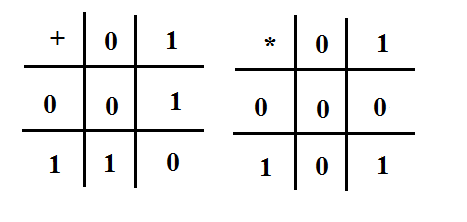
\includegraphics[scale=0.6]{1-1.PNG}
\end{figure}\\
Факт: $(-1)\cdot(-1) = 1$ \\
Док-во:Докажем сначала 2 свойства:
а) $-x = (-1)\cdot x$\\
$x+(-1)\cdot x = (1+(-1))\cdot x = 0\cdot x = x\cdot 0 = 0$ и утверждение следует из единственности противоп. элемента\\
б)$(-1)(-x) = x$ следует из (a) и единственности элемента $x$, противоположного $-x$\\
Тогда докажем, что для любого x верно:
$(-x)(-x) = x\cdot x$\\
$(-x)(-x) = ((-1)\cdot x)(-x)=(x\cdot (-1))(-x) = x((-1)(-x)) = x\cdot x$\\
Мы последовательно воспольз. двумя свойствами, а также коммутативностью и ассоциативностью умножения. \\
Определение: комплексное число $z = a +bi$ - это упорядоченная пара вещественных чисел $a$ и $b$ ($a = Re z$ - вещ.часть, $b = Im z$ - мнимая часть)\\
\begin{figure}[h!]
\centering
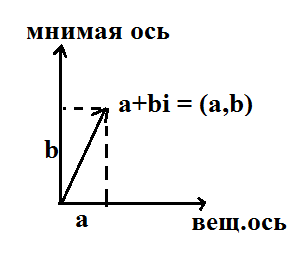
\includegraphics[scale=0.6]{1-2.PNG}
\end{figure}\\
Определение сложения: $z_1 = a_1 + b_1 i, z_2 = a_2 + b_2 i\\
z_1 + z_2 = (a_1 + a_2) + (b_1 + b_2)i$\\
Определение умножения: $z_2 \cdot z_2 = (a_1 \cdot a_2 - b_1 \cdot b_2) + (a_1 \cdot b_2 + b_1 \cdot a_2)i$\\
Геом.смысл: поворот на $90^{o}$ против часовой стрелки\\
\begin{figure}[h!]
\centering
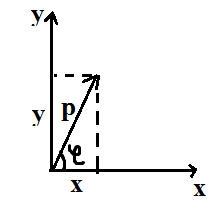
\includegraphics[scale=0.6]{1-3.PNG}
\end{figure}\\
Полярные координаты: $\rho = \sqrt{x^2 +y^2}$
$$\begin{cases}
x = \rho \cdot \cos{\phi}  \\
y = \rho \cdot \sin{\phi}
\end{cases}$$\\
\begin{figure}[h!]
\centering
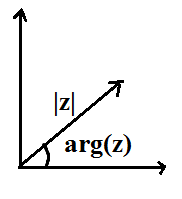
\includegraphics[scale=0.6]{1-4.PNG}
\end{figure}\\
$|z| = \sqrt{Re z^2 + Im z^2},\ \
|z-1| = \sqrt{Re (z-1)^2 +Im (z-1)^2} = \sqrt{Re (z -1)^2 + Im z^2}\\
|z-1| = \sqrt{(a-1)^2 +b^2}, z = a+bi$\\
Тригонометрическая форма комплексного числа: $z = |z|(\cos{(arg z)} + i\sin{(arg z)} = |z| (\cos{\phi} + i\sin{\phi}) = |z|\cdot e^{i\phi}$\\
Утверждение: $z_1 = {\rho}_1 \cdot e^{i \phi}, z_2 = {\rho}_2 \cdot e^{i \psi} \Longrightarrow z_1 \cdot z_2 = {\rho}_1 \cdot {\rho}_2 \cdot e^{i(\phi + \psi}\\
{\rho}_1 = |z_1|, \phi = arg(z_1), {\rho}_2 = |z_2|, \psi = arg(z_2)$\\
Модули перемножаются, аргументы складываются\\
Основная теорема алгебры: Уравнение $a_n x^n + a_{n-1} x^{n-1}+...+a_0 = 0 (a_i \in \mathbb{C}, a_n \neq 0)$ имеет $n$ комплексных решений.

%2 done 
\item \textbf{Определения: сложение векторов и умножение на число в вещественном координатном пространстве, 8 свойств (аксиомы векторного пространства), линейное отображение, матрицы и произведение матриц. Примеры: одномерный случай, матрица умноженная на столбец дает столбец, матрица для поворота на 90 градусов и для поворота на произвольный угол. Каждое линейное отображение задается матрицей.}\\

Опр (координатное пр-во ${\mathbb{R}}^n$): ${\mathbb{R}}^n = \{(x_1,...,x_n)|x_i \in\mathbb{R}\}$, где $(x_1,...,x_n)$ - упорядоченные наборы из n чисел\\
n - размерность пр-ва ${\mathbb{R}}^n$\\
$(x_1,...,x_n) =(y_1,...,y_n) \Leftrightarrow x_1 =y_1, ... , x_n = y_n$\\
Опр(сложение векторов и умножение на число):\\
I) $x = (x_1 , ... , x_n)$ и $y = (y_1, ... , y_n$)\\
$x+y = (x_1+y_1 , ... y_1+y_n$)\\
Очевидно: (1) x+y = y+x (коммутативность)\\
(2) (x+y)+z = x+(y+z) (ассоциативность)\\
Нулевой вектор: 0 = (0,...,0)\\
(3) x+0 = x\\
(4)$\forall \in {\mathbb{R}}^n \ \exists y \in {\mathbb{R}}^n \  x+y = 0$\\
Противополодный вектор $y = (-x_1, ..., -x_n)$\\

II) $\lambda \in \mathbb{R}\\
\lambda x = (\lambda x_1, ..., \lambda x_n)\\
(5)\lambda (x+y) = \lambda x + \lambda y\\
(6) (\lambda + \mu)x = \lambda x + \mu x\\
(7) 0 \cdot x = 0\\
(8) 1 \cdot x = x$\\
Опр: Отображение $f: \mathbb{R}^n \longrightarrow \mathbb{R}$ называется линейным, если $\forall x,y \in \mathbb{R}^n, \forall \lambda \in \mathbb{R}$:\\
$(1)f(x+y)=f(x)+f(y)$\\
$(2)f(\lambda x) = \lambda f(x)$\\
Опр: Матрица размера $n \times m$ над $\mathbb{R}$ - это такая таблица, в которой $n$ строк и $m$ столбцов\\
\begin{figure}[h!]
\centering
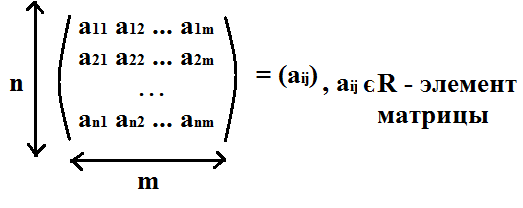
\includegraphics[scale=0.6]{2-1.PNG}
\end{figure}\\
Опр:  $A = (a_{ij}), i = 1,...,n; j = 1,..., m$\\
$B = (b_{kl}), k = 1,...,m; l = 1,..., p$\\
$A$ -размера $n\times m, B$ - размера $m\times p$\\
Тогда можем определить матрицу $C = (i, l)$\\
$C_{il} = \overset{m}{\underset{j=1}{\sum}} a_{ij} \cdot b_{jl} = a_{i1}\cdot b_{1l} + a_{i2}\cdot b_{2l} + ... + a_{im}\cdot b_{ml}$\\
\begin{figure}[h!]
\centering
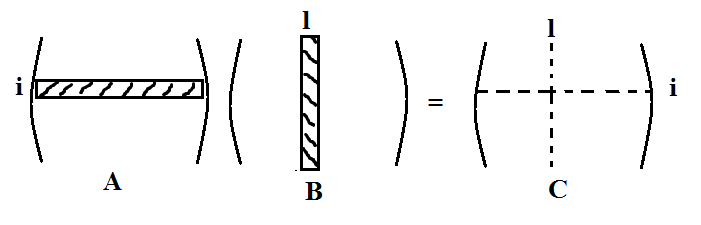
\includegraphics[scale=0.6]{2-2.PNG}
\end{figure}\\
Пример 1: $f: \mathbb{R} \longrightarrow \mathbb{R}$ - линейно, если $f(x) = kx$ для некоторого $k\in \mathbb{R}$\\
В самом деле, если $f$ - линейно, то $f(x) = f(x\cdot 1) = x\cdot f(1)$, где $k = f(1)$\\
Наоборот: $k(x+y) = kx + ky\\
k(\lambda x) = \lambda (kx)$\\
Пример 2: $\begin{pmatrix}
a_{11}  &  a_{12}  & ...  &  a_{1m} \\
a_{21}  &  a_{22}  & ...  &  a_{2m} \\
... \\
a_{n1}  &  a_{n2}  & ...  &  a_{nm} \\
\end{pmatrix}
\begin{pmatrix}
x_1 \\
x_2 \\
... \\
x_m \\
\end{pmatrix} = 
\begin{pmatrix}
y_1 \\
y_2 \\
... \\
y_n \\
\end{pmatrix}$\\
$y_1 = a_{11} x_1 + a_{12} x_2 + ... + a_{1m} x_m\\
y_2 = a_{21} x_1 + a_{22} x_2 + ... + a_{2m} x_m\\
y_1 = a_{n1} x_1 + a_{n2} x_2 + ... + a_{nm} x_m$\\

Пример 3: поворот на $90^{o}$\\
$y_1 = -x_2, y_2 = x_1$\\
$\begin{pmatrix}
y_1 \\
y_2 \\
\end{pmatrix}
=
\begin{pmatrix}
0 & -1 \\
1 & 0 \\
\end{pmatrix}
\begin{pmatrix}
x_1 \\
x_2 \\
\end{pmatrix}$\\
\begin{figure}[h!]
\centering
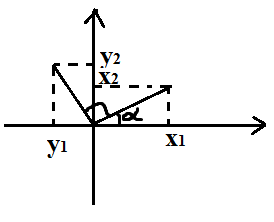
\includegraphics[scale=0.6]{2-3.PNG}
\end{figure}\\
Пример 4: поворот на угол $\phi$
$x_1 = r \cos{\alpha}, x_2 = r \sin{\alpha}\\
y_1 = r \cos{(\alpha + \phi)} = r(\cos{\alpha} \cos{\phi} - \sin{\alpha} \sin{\phi})\\
y_2 = r \sin{(\alpha + \phi)} = r(\sin{\alpha} \cos{\phi} + \cos{\alpha} \sin{\phi})\\
y_1 = x_1 \cos{\phi} - x_2 \sin{\phi}\\
y_2 = x_2 \sin{\phi} + x_2 \cos{\phi}$\\
$\begin{pmatrix}
y_1 \\
y_2 \\
\end{pmatrix}
=
\begin{pmatrix}
\cos{\phi} & -\sin{\phi} \\
\sin{\phi} & \cos{\phi} \\
\end{pmatrix}
\begin{pmatrix}
x_1 \\
x_2 \\
\end{pmatrix}$\\
Опр: Координатные векторы в $\mathbb{R}\\
e_i = (0,..., 1, 0, ..., 0), 1$ стоит на $i$-ом месте\\
$x = (x_1,...,x_n) = x_1 e_1 + x_2 e_2 +...+ x_m e_m$\\
Теорема: любое линейное отображение $f: \mathbb{R}^m \longrightarrow \mathbb{R}^n$ имеет вид $f(x) = Ax$ для некоторой матрицы $A$ размером $n\times m$\\
Док-во: $f(x) = f(x_1 e_1 + x_2 e_2 +...+ x_m e_m) = x_1 f(e_1) + ...+ x_m f(e_m)$\\
$f(e_i) = \begin{pmatrix}
\lambda_{i1} \\
\lambda_{i2} \\
... \\
\lambda_{in} \\
\end{pmatrix} 
= \lambda_{i1} \overset{\thicksim}{e_1} + ... + \lambda_{in} \overset{\thicksim}{e_n}= \overset{n}{\underset{j=1}{\sum}} \lambda_{ij} \overset{\thicksim}{e_j}
\Longrightarrow f(x) = \overset{m}{\underset{i=1}{\sum}} \overset{n}{\underset{j=1}{\sum}} x_i \lambda_{ij} \overset{\thicksim}{e_j} = \overset{n}{\underset{j=1}{\sum}} (\overset{m}{\underset{i=1}{\sum}} x_i \lambda_{ij}) \overset{\thicksim}{e_j}$\\
Пусть $a_{ij} = \lambda_{ji}\\
y_j = \overset{m}{\underset{i=1}{\sum}} a_{ji} x_i\\
y = Ax$




%3 done 
\item \textbf{Определения: скалярное произведение, длина, расстояние, метрика, площадь, объём. Примеры: евклидова метрика, метрика такси. Билинейность скалярного произведения. Вычисление косинуса угла между векторами через скалярное произведение. Вычисление площади параллелограмма через равносоставленность.}\\
Опр: Длина вектора $|\overline{v}| = \sqrt{x_0^2 + y_0^2}\\
(1) |\overline{v}| \textgreater 0$, если $\textgreater \neq 0$ - положительность\\
(2) $|a \overline{v}| = |a|\cdot |\overline{v}|, a\in \mathbb{R}$ - однородность\\
(3) $|\overline{v}| + |\overline{u}| \geq |\overline{v} + \overline{u}|$ - неравенство треугольника\\
Опр: Функция $|| \cdot||: \mathbb{R}^n \longrightarrow \mathbb{R}$ называется нормой, если выполняются свойства (1)-(3)\\
$v \longrightarrow ||v||$ - вектор в число\\
длина $\longleftrightarrow$ норма, расстояние $\longleftrightarrow$ метрика\\
Опр: расстояние между двумя точками это $l = \sqrt{(x_1 - x_2)^2 + (y_1 - y_2)^2}$ (она же евклилова метрика)
Метрика такси:
$d(A,B) = |x_2 - x_1| + |y_2-y_1|$\\
Опр: скалярное произведение $(\overline{v_1}, \overline{v_2}) = x_1 x_2 + y_1 y_2\\
\cos{\phi} = \frac{(\overline{v_1}, \overline{v_2})}{|\overline{v_1}| \cdot |\overline{v_2}|}$\\
Опр: $f(u,v)\in \mathbb{R}$ билинейна, если:\\
$(1) f(u, v_1 + v_2) = f(u,v_1) + f(u,v_2)\\
(2)f(u_1 + u_2, v) = f(u_1,v) + f(u_2, v)\\
(3) f(u, \lambda v) = \lambda f(u,v)\\
(4)f(\lambda u, v) = \lambda f(u,v)$\\
Пример: $f(\lambda u, \lambda v) = {\lambda}^2 f(u,v)$\\
\textbf{Площадь ориентированная}
$\omega (\overline{v_1}, \overline{v_2}) = - \omega (\overline{v_2}, \overline{v_1})\\
\overline{v_1} = \overline{v_2} = \omega (v_1, v_1) = 0$\\
\begin{figure}[h!]
\centering
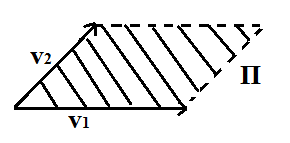
\includegraphics[scale=0.6]{3-1.PNG}
\end{figure}\\
Свойства площади:\\
S: многоугольники $\longrightarrow \mathbb{R}\\
(1)S(\lambda \Pi) = {\lambda}^2 S(\Pi)$\\
(2)$S$(единич.квадрата) $= 1$\\
(3)$S({\Delta}_1 \cup {\Delta}_2) = S({\Delta}_1)+S({\Delta}_2)$ - аддитивность \\
(4) $\omega(\lambda \overline{v_1}, \overline{v_2}) = \lambda \omega(\overline{v_1}, \overline{v_2})\\
(5)\omega(\overline{v_1},\lambda  \overline{v_2}) = \lambda \omega(\overline{v_1}, \overline{v_2})$\\
$((4) и (5)$ - билинейна относительно сложения)
(6)$\omega (v_1, v_1) = 0 \\
(7)\omega ((1,0),(0,1)) = 1\\
Из (4), (5) \Longrightarrow$ площадь прямоугольника\\
$\omega ((x_1,0),(0,y_2)) = x_1 y_2\\
(x,y) \longrightarrow (2x, \frac{y}{2})$ - сохраняет $S$\\
\begin{figure}[h!]
\centering
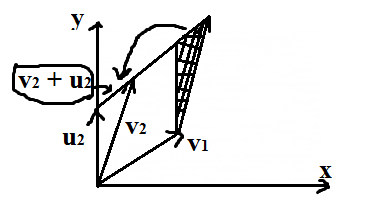
\includegraphics[scale=0.8]{3-2.PNG}
\end{figure}\\
$\overline{v_2} - \overline{u_2} - коллинеарен \overline{v_1}\\
\omega (\overline{v_1}, \overline{v_2}) = \omega (\overline{v_1}, (\overline{v_2} - \overline{u_2}) + \overline{u_2}) = \omega (\overline{v_1}, (\overline{v_2} - \overline{u_2})) + \omega (\overline{v_1}, \overline{u_2}) = \omega (\overline{v_1}, \overline{u_2})$ чтд


%4 done 
\item \textbf{Определения: группа перестановок, инверсии (беспорядки), длина и знак перестановки, транспозиции и циклы. Связь между знаком перестановки и ориентированным объемом параллелепипеда. Перестановка раскладывается в произведение непересекающихся циклов. Задача об арестантах. Группы симметрий правильных многоугольников, тетраэдра и куба.}\\
\textbf{Группа перестановок $S_n$}\\
Опр: перестановка $\sigma$ на $n$ элементах - это взаимнооднозначное отображение $\sigma: \{1,...,n\} \longrightarrow \{1,...,n\}$\\
$\begin{pmatrix}
1 & 2 & ... & n \\
\sigma (1) & \sigma (2)\ & ... & \sigma (n)\\
\end{pmatrix}$\\
Пример: $n = 4\\
\sigma: 1\longrightarrow 2\\
2\longrightarrow 3\\
3 \longrightarrow 4\\
4\longrightarrow 1\\
\sigma: \begin{pmatrix}
1 & 2 & 3 & 4\\
2 & 3 & 4 & 1\\
\end{pmatrix}\\
|S_n| = n!$\\
\textbf{Умножение:} $\sigma: \{1,...,n\} \longrightarrow \{1,...,n\}\\
\tau: \{1,...,n\} \longrightarrow \{1,...,n\}\\
\sigma o \tau = \sigma (\tau (x))\\
(\sigma \tau)\pi = \sigma (\tau \pi)$ - ассоциативность \\
\begin{figure}[h!]
\centering
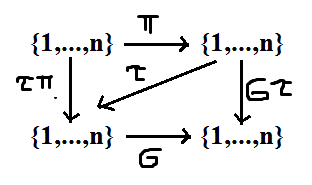
\includegraphics[scale=0.6]{4-1.PNG}
\end{figure}\\
Опр: $id$ - единичная перестановка (тождественное отображение)\\
$id = \begin{pmatrix}
1 & 2 & ... & n\\
1 & 2 & ... & n\\
\end{pmatrix}$\\
Утверждение: для любое $\sigma \in S_n$ существует ${\sigma}^{-1} \in S_n$ такая, что $\sigma o {\sigma}^{-1} = {\sigma}^{-1} o \sigma = id$\\
Док-во: ${\sigma}^{-1}$ - отображение обратное к $\sigma$\\
Пример: $\sigma = \begin{pmatrix}
1 & 2 & 3 & 4 & 5\\
2 & 3 & 5 & 4 & 1\\
\end{pmatrix}\\
{\sigma}^{-1} = \begin{pmatrix}
2 & 3 & 5 & 4 & 1\\
1 & 2 & 3 & 4 & 5\\
\end{pmatrix}$\\
\textbf{Знак перестановки}
Хотим: $\sigma \longrightarrow sgn(\sigma) = \pm 1\\
sgn(\sigma) = 1 \Longleftrightarrow \sigma$ - четная \\
$sgn(\sigma) = -1 \Longleftrightarrow \sigma$ - нечетная \\
$sgn(\sigma \tau) = sgn(\sigma)  \cdot sgn(\tau) \Longleftrightarrow$ знак мультипликативен \\
Опр 1: инверсия (беспорядок) для перестановки $\sigma$ - это пара $(i,j)$ такая, что:\\
$(1) i \textless j \\
(2) \sigma (i) \textgreater \sigma (j)$\\
Длина перестановки $k =$ число инверсий \\
Знак $sgn(\sigma) = (-1)^{k-1} или sgn(\sigma) = (-1)^{\text{количество инверсий}}$\\
Пример: \begin{figure}[h!]
\centering
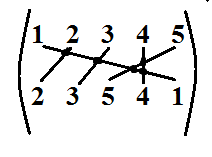
\includegraphics[scale=0.6]{4-2.PNG}
\end{figure}\\
$5$ инверсий, $(-1)^5 = -1$\\
Опр 2: $\sigma = {\tau}_1 o {\tau}_2 o ...o {\tau}_n$ - произведение транспозиций\\
Транспозиция $(i,j) = \begin{pmatrix}
1 & 2 & ... & i & j & ...  n\\
1 & 2 & ... & j & i & ...  n\\
\end{pmatrix}\\
(ij)^2 = id$\\
Пример: $id = (35)(23)(12)\sigma = \begin{pmatrix}
1 & 2 & 3 & 4 & 5\\
1 & 2 & 3 & 4 & 5\\
\end{pmatrix}\\
\sigma = (12)(23)(35)\\
sgn(\sigma) = (-1)^3 = -1$\\
Утверждение: $sgn(\sigma \tau) = sgn(\sigma) \cdot sgn(\tau)$\\
Док-во: $\sigma = {\tau}_1 \cdot ... \cdot {\tau}_l$
$\sigma \tau = {\tau}_1 \cdot ... \cdot {\tau}_l \cdot {\pi}_1 \cdot ... \cdot {\pi}_k$\\
$(-1)^{k+l} = (-1)^k \cdot (-1)^l$\\
Опр: $l_i = \begin{pmatrix}
0 & 0 & ... & 0 & 1 & 0 & ... & 0\\
 & & & & i & & & \\
\end{pmatrix}$
$V(\Pi (l_1, ..., l_n)) = 1\\
V(\Pi (l_{\sigma (1)},..., l_{\sigma (n)})) = sgn (\sigma)$\\
\textbf{Задача об арестантах:}  Тюремщик идет в секретную комнату и подготавливает 100 коробок с крышками. На каждую коробку он наносит числа с нумерацией от 1 до 100. Затем он приносит 100 бумажных табличек, по числу заключенных, и нумерует эти таблички от 1 до 100. После этого он перемешивает 100 табличек и помещает в каждую коробку по одной табличке, закрывая крышку. Заключенные не видят, как тюремщик выполняет все эти действия. Соревнование начинается, тюремщик отводит каждого заключенного по одному в комнату с коробками и говорит заключенным, что они должны найти коробку, в которой будет находиться табличка с номером заключенного. Заключенные пытаются найти табличку со своим номером, открывая коробки. Каждому разрешается открыть до 50-ти коробок; если каждый из заключенных найдет свой номер, то заключенных отпустят, если хотя бы один из них не найдет свой номер за 50 попыток, то все заключенные умрут.\\
После открытия коробки заключенным и проверки им таблички она помещается обратно в коробку и крышка снова закрывается;\\
Местами таблички менять нельзя;\\
Заключенные не могут оставлять друг другу подсказки или как-то взаимодействовать друг с другом после начала испытания;\\
Заключенным разрешается обсудить стратегию до начала испытания.\\
\\
\textbf{Решение:} Стратегия крайне легкая. Первый из заключенных открывает коробку с тем номером, который написан на его одежде. Например, заключенный номер 78 открывает коробку с номером 78. Если он находит свой номер на табличке внутри коробки, то это здорово! Если нет, то он смотрит номер на табличке в «своей» коробке и затем открывает следующую коробку с этим номером. Открыв вторую коробку, он смотрит номер таблички внутри этой коробки и открывает третью коробку с этим номером.\\
В каждой коробке по одной табличке - и эта табличка уникальна. Это означает, что табличка находится в коробке с тем же номером, или она указывает на другую коробку. Так как все таблички уникальны, то для каждой коробки есть только одна табличка, указывающая на нее (и всего один путь, как добраться до этой коробки).Если поразмыслить над этим, то коробки образуют замкнутую круглую цепочку. Одна коробка может быть частью только одной цепочки, так как внутри коробки только один указатель на следующую и, соответственно, в предыдущей коробке только один указатель на данную коробку (программисты могут увидеть аналогию со связанными списками).\\
Если коробка не указывает на саму себя (номер коробки равен номеру таблички в ней), то она будет в цепочке. Некоторые цепочки могут состоять из двух коробок, некоторые длиннее. Так как все заключенные начинают с коробки с тем же номером, что и на их одежде, они, по определению, попадают на цепочку, которая содержит их табличку (есть всего одна табличка, которая указывает на эту коробку).Исследуя коробки по этой цепочке по кругу, они гарантированно в конечном итоге найдут свою табличку.\\
Для того, чтобы все заключенные прошли испытание, максимальная длина цепочки должна быть меньше, чем 50 коробок. Если цепочка длиннее, чем 50 коробок, заключенные, имеющие номера из этих цепочек провалят испытание — и все заключенные будут мертвы.\\
Если максимальная длина самой длинной цепочки меньше, чем 50 коробок, тогда все заключенные пройдут испытание!\\
Итак, что нам нужно, чтобы выяснить вероятность существования длинной цепочки?Для цепочки с длиной $l$, вероятность того, что коробки будут вне этой цепочки равна $C_{100}^l$ \\
В этой коллекции чисел существует $(l-1)!$ способов расположить таблички.\\
Оставшиеся таблички могут быть расположены $(100-l)!$ способами (не забываем, что длина цепочки не превосходит $50$).\\
Учитывая это, число перестановок, которые содержат цепочку точной длины $l: (>50): C_{100}^l \cdot (l-1)! \cdot (100-l)! = \frac{100!}{l}$\\
Выходит, есть $100(!)$ способов раскладок табличек, так что вероятность существования цепочки длиной $l$ равно $1/l$. Кстати, этот результат не зависит от количества коробок.\\
Как мы уже знаем, может быть только один вариант, при котором существует цепочка длиной $> 50$, так что вероятность успеха рассчитывается по данной формуле:
$Win = 1 - [\frac{1}{51} + \frac{1}{52} + \frac{1}{53}+...+ \frac{1}{98} + \frac{1}{99} + \frac{1}{100}] \approx 0.3118$\\
$31.18$ процентов — вероятность того, что размер самой длинной цепочки будет меньше $50$ и каждый из заключенных сможет найти свою табличку, учитывая предел в $50$ попыток.
\\
Опр: k-цикл - это перестановка: \\
\begin{figure}[h!]
\centering
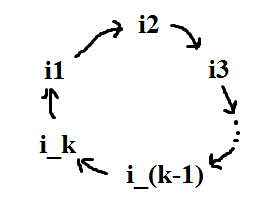
\includegraphics[scale=0.6]{4-3.PNG}
\end{figure}\\
$j \neq i_1, ..., i_k\\
\sigma (j) = j$
Теорема: каждая перестановка единственным образом раскладывается в произведение непересекаемых циклов\\
Пример: $\begin{pmatrix}
1 & 2 & 3 & 4 & 5 & 6 & 7 & 8\\
3 & 5 & 7 & 4 & 8 & 2 & 6 & 1\\
\end{pmatrix}$\\
\begin{figure}[h!]
\centering
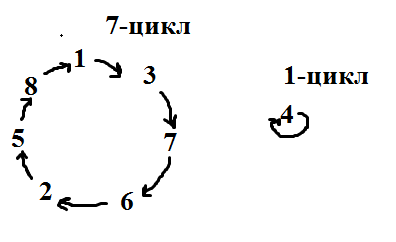
\includegraphics[scale=0.6]{4-4.PNG}
\end{figure}\\
Док-во: I. $1 \longrightarrow \sigma (1) \longrightarrow {\sigma}^2 (1) \longrightarrow ... \longrightarrow {\sigma}^{k-1} (1) \longrightarrow {\sigma}^k (1) = 1$ (но не равно какому-нибудь ${\sigma}^2 (1)) \Longrightarrow k$-цикл, $(1 \sigma (1) {\sigma}^2 ... {\sigma}^{k-1} (1) {\sigma}^k (1) )$\\
II. $j\neq 1, \sigma (1), ..., {\sigma}^{k-1} (1)$\\
Применим $I$ к $j$\\
\begin{figure}[h!]
\centering
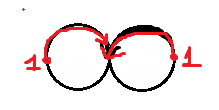
\includegraphics[scale=0.6]{4-5.PNG}
\end{figure}\\
Следствие: $\sigma =$ цикл длины $k_1 \cdot$ цикл длины $k_2 \cdot$ ... $\cdot$ цикл длины $k_s$\\
$sgn(\sigma) = sgn($цикл длины $k_1) \cdot ($цикл длины $k_2) \cdot ... \cdot ($цикл длины $k_s) = (-1)^{k_1 + k+2 + ... + k_s - s}$\\
\textbf{Связь между знаком перестановки и ориентированным объемом параллелепипеда:}\\
Параллелепипед однозначно определяется заданием трех его направленных ребер, выходящих из одной вершины. Ориентированным параллелепипедом называется параллелепипед, у которого упорядочены три ребра, выходящие из одной вершины.\\
Будем говорить, что невырожденный ориентированный параллелепипед П имеет положительную ориентацию, если он одинаково ориентирован с базисным параллелепипедом; если же эти параллелепипеды имеют противоположные ориентации, то параллелепипед П имеет отрицательную ориентацию.\\
Объемом невырожденного ориентированного параллелепипеда, находящегося в ориентированном пространстве, называется число, равное по абсолютной величине объему параллелепипеда с ребрами (a,b,c), положительное, если упорядоченная тройка направленных ребер a,b, c имеет положительную ориентацию, и отрицательное, если упорядоченная тройка имеет отрицательную ориентацию.\\
Объем ориентированного параллелепипеда, построенного на векторах a, b, c обладает следующим свойством:\\
$abc = bca = cab = -bac = -acb = -cba$ (т.е. от круговой перестановки множителей он не меняется, а при нарушении кругового порядка множителей меняет знак, сохраняя абсолютную величину, либо если перестановка четная, то знак +, если перестановка нечетная, то знак -)
\textbf{Группы симметрий правильных многоугольников, тетраэдра и куба}\\
Группа диэдра - группа симметрий правильных многоугольников\\
Это либо поворот, либо отражение по оси симметрии. Ибо веришины переходят в вершины, а стороны в стороны.
$D_n = 2n, n - поворотов на углы k\cdot \frac{2\pi}{n}$, где $k = 0, 1, ..., n-1$, и еще $n$ - симметрии относительно осей, т.к. (1) случай. Пусть у нас n-угольник и n=2k+1. Осей симметрии в этом случае ось симметрии проходит через вершину и сторону противоположную ей, значит 2k+1 (=n) осей. (2) Пусть n=2k, тогда оси симметрии это прямые проходящие через противоположные вершины $\Rightarrow$ k осей и еще проходящие через середины противоположных сторон $\Rightarrow$ еще k осей. Итог: 2k (=n)\\
\begin{figure}[h!]
\centering
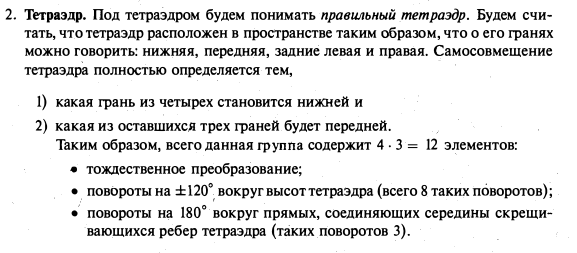
\includegraphics[scale=1.1]{4-6.PNG}
\end{figure}\\
\begin{figure}[h!]
\centering
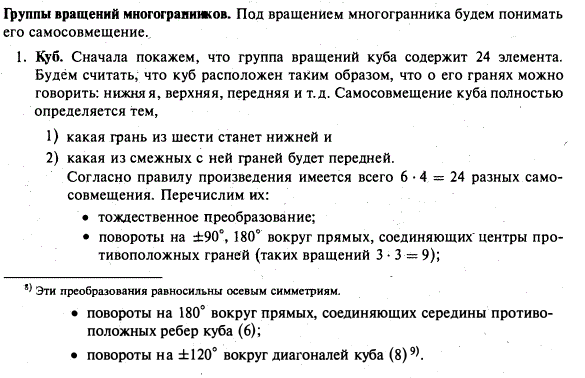
\includegraphics[scale=1.1]{4-7.PNG}
\end{figure}\\


%5 done
\item \textbf{Определения: делимость в кольцах, простые и неприводимые элементы, деление с остатком. Примеры: целые числа, гауссовы целые числа, неприводимый и не простой элемент в $\bb{Z}[\sqrt{5}]$, кольцо многочленов с коэффициентами в поле. Решето Эратосфена. Алгоритм Евклида, цепные дроби и представление НОД($a,b$) в виде линейной комбинации чисел $a$ и $b$. Основная теорема арифметики. Деление с остатком в гауссовых целых числах.}\\
R - ассоциативное коммутативное кольцо с единицей.\\
Пример: $\mathbb{Z}$, $\mathbb{Z}[i] = {a + bi \ | \ a,b \in \mathbb{Z} }$ целые гауссовые числа, $\mathbb{Z}[\sqrt{5}] = { a + b\sqrt{5} \ | \ a, b \in \mathbb{Z}}$. \\
Пример кольца многочленов с коэффициентами в поле: это многочлен степени $n$ с коэффициентами в поле $\mathbb{F}$ ($x^2 + x + 1$) \\
\textit{Опр.} $a, b \in R$. a \textbf{делится} на b ($\Longleftrightarrow$ b \textbf{делит} a) $\exists c \in R : a = b \cdot c$ $(a \mathrel{\vdots} b \Longleftrightarrow b | a)$. \\
\textit{Опр.} $p \in R$ \textbf{неприводимый}, если $p$ делится только на себя и на обратимые элементы. \\
\textit{Опр.} $p \in R$ \textbf{простое}, если $\forall a,b \in R$ из того, что $p | ab \Longrightarrow p|a$ или $p|b $  (упр. простые элементы неприводимые). \\
Пример: $2 \in \mathbb{Z}[\sqrt{5}] $ неприводимый, но не простой. \\
\textbf{Решето Эратосфена} - алгоритм нахождения всех простых чисел до некоторого целого числа n, который приписывают древнегреческому математику Эратосфену Киренскому. Как и во многих случаях, здесь название алгоритма говорит о принципе его работы, то есть решето подразумевает фильтрацию, в данном случае фильтрацию всех чисел за исключением простых. По мере прохождения списка нужные числа остаются, а ненужные (они называются составными) исключаются. \\
\textbf{Делимость с остатком в гауссовых числах.} \\
Любое гауссовое число $u$ можно разделить с остатком на любое ненулевое гауссово число $v$, то есть представить в виде: $u = vq + r,$ где $q$ и остаток $r$ - гауссовы числа, причем $|r| < |v|.$\\
Пример: $7 + 2i = (3 - i)(2 + i) + i = (3 - i)(1 + i) + 3 = (3 - i)(2 + 2i) + (-1 - 2i).$ \\
\textbf{Алгоритм Евклида} -  эффективный алгоритм для нахождения наибольшего общего делителя двух чисел. \\
НОД($a, b$) = $(a,b)$, $a > b$, $a = b q_1 + r_1$. (упр. НОД($a,b$) = НОД($b, r_1$) $r_1 < b$. \\
$\blacktriangleleft$ $(a,b) = (b, r_1) = ... = (r_n, 0) = r_n = x \cdot a + y \cdot b, x,y \in \mathbb{Z}$ $\blacktriangleright$ \\
Цепные дроби $\sqrt{2} = 1 + (\sqrt{2} - 1) = 1 + \frac{1}{\sqrt{2}+1} = 1 + \frac{1}{2 + \frac{1}{2 + \frac{1}{2 + \frac{1}{2 + ...}}}}$ \\
\textbf{Утв.} $a,b \in \mathbb{Z} \ \exists \ x,y \in \mathbb{Z} \ (a, b) = ax + by$.\\ \underline{Лемма}: $p$ - неприводимое $\Longleftrightarrow p | ab \Longrightarrow p|a$ или $p|b$ для $\mathbb{Z}$. \\
$\blacktriangleleft $ $(p, a) \neq p \Longrightarrow (p, a) = 1 \Longrightarrow 1 = ax + py \\
b = abx + pby (ab$ не делится на $p, pb$ делится на $p \Longrightarrow b$ не делится на $p$. $\blacktriangleright$ \\
$\textit{\textbf{Основная теорема арифметики}}$: Каждое необратимое целое число раскладывается единственным образов в произведение $n = \pm p^{k_1}_1 \cdot p^{k_2}_2 \cdot ... \cdot p^{k_s}_s$ ($0 < p_1 < p_2 < ... < p_s$).\\
$\blacktriangleleft$ Существование: (1) $n$ - простое $\Longrightarrow n = p$ \\
(2) $n$ - не простое $\Longrightarrow \ \exists \ m \neq n, \pm 1 \ | \ n = mk \Longrightarrow m < n \Longrightarrow$ (a) $m$ - простое или  (b) можем разложить и т.д \\
$n > m_1 > m_2 ... > p$ по принципу наименьшего элемента у $n$ есть простой делитель $p$. $\blacktriangleright$\\
Единственность: $\blacktriangleleft p^{k_1}_1 ... p^{k_s}_s = q^{l_1}_1 ... q^{l_t}_t$\\
$p_1 | q^{l_1}_1 ... q^{l_t}_t \Longrightarrow p_1 | q^{l_1}_1 \Longrightarrow p_1 = q_1$\\
Индукция по $k_1 + ... + k_s \blacktriangleright$


%6 done
\item \textbf{Определения: векторное пространство, векторы, скаляры, линейная комбинация, линейная зависимость, элементарные преобразования строк матрицы. Примеры: координатное векторное простарнство. Метод Гаусса. Приведение матрицы к стандратной ступенчатой форме преобразованиями строк, решение систем линейных уравнений и поиск линейной зависимости между векторами.}\\
\textit{Опр.} \textbf{Векторное пространство} $V$ над полем $\mathbb{F}$ - это множество с двумя операциями: \\
(1) сложение $\exists \ u + v \in V \ \forall u, v \in V $\\
(2) умножение на скаляр $\exists \ \lambda v \in V \ \forall \lambda \in \mathbb{F}, v \in V$, удовлетворяющими 8-ми аксиомам. \\
Элементы поля $\mathbb{F}$ = скаляры \\
Элементы пр-ва $V$ = векторы \\
\textbf{Аксиомы векторного пространства:}\\
(1) $u + v = v + u$ [сложение коммутативно]\\
(2) $\exists \ 0 \in V : 0 + v = v$ [существование 0] \\
(3) $\forall v \in V \ \exists \ (-v) : v + (-v) = 0 \in V$ [обратный элемент] \\
(4) $u + (v + w) = (u + v) + w$ [ассоциативность] \\
(5) $\lambda (\mu v) = (\lambda \mu) v$ \\
(6) $1 \cdot v = v \ \forall v \in V, 1\in \mathbb{F}$\\
(7) $(\lambda + \mu) v = \lambda v + \mu v$ \\
(8) $\lambda(u + v) = \lambda u + \lambda v$ \\
\textit{Опр.} \textbf{Линейная комбинация векторов} $v_1, ... , v_n$ с коэффициентами $\lambda_1, ... , \lambda_n $ = $ \lambda_1 v_1 + ... + \lambda_n v_n$\\
\textit{Опр.} \textbf{Координатное пространство} $\mathbb{F}_n =$ \{$(x_1, ... , x_n) | x_i \in \mathbb{F}$ \} \\
$u = (x_1, ... , x_n); v = (y_1, ... , y_n) \Rightarrow u + v = (x_1 + y_1, ... , x_n + y_n); \lambda u = (\lambda x_1, ... , \lambda x_n)$ \\
\textit{Опр.} \textbf{Элементарные преобразования матрицы} - это такие преобразования матрицы, в результате которых сохраняется эквивалентность матриц. Таким образом, элементарные преобразования не изменяют множество решений системы линейных алгебраических уравнений, которую представляет эта матрица. \\
\textbf{Преобразования строк:}\\
I. $R_i \rightarrow R_i + \lambda R_j$ [обратимое преобразование] \\
II. $R_i \leftrightarrow R_j$ [транспозиция]\\
III. $R_i \rightarrow aR_i \ a \neq 0 \ a \in \mathbb{F}$ \\
\textbf{Метод Гаусса} - приведение матриц к стандартному ступенчатому виду. \\
$\begin{cases}
    a_{11} x_1 + ... + a_{1n} x_n = b_1
    \\
    a_{21} x_1 + ... + a_{2n} x_n = b_2
    \\
    ...
    \\
    a_{m1} x_1 + ... + a_{mn} x_n = b_m
\end{cases}$

$A = 
\begin{pmatrix}
    a_{11} ... a_{1n} \\
    ... ... ... \\
    a_{m1} ... a_{mn}
\end{pmatrix}$
$X = 
\begin{pmatrix}
    x_1 \\
    ... \\
    x_n
\end{pmatrix}$
$B = 
\begin{pmatrix}
    b_1 \\
    ... \\
    b_m
\end{pmatrix} \\
AX = B$ \\
\textit{\textbf{Теорема:}} любую матрицу можно привести элементарными преобразованиями строк к следующему виду \\
$\begin{pmatrix}
    0 .. 0 1 x .. x .. 0 x .. 0 x 0 x .. \\
    0 .. 0 0 0 .. 0 .. 1 .. .. 0 x 0 x .. \\
    0 .. 0 0 0 .. 0 .. 0 .. .. 1 x 0 x .. \\
    .. .. .. .. .. .. .. .. .. .. .. .. .. .. .. .. \\
    0 0 0 0 0 0 0 0 0 0 0 0 0 0 0 0 
\end{pmatrix}$, где x - любое число \\
\textit{\textbf{Доказательство:}}\\
$A = m \times \ n \\
\begin{pmatrix}
    a_{11} \\
    ... \\
    a_{m1}
\end{pmatrix}$
возьмем самый левый ненулевой столбец \\
$a_{i1} \neq 0$ \\
Применим преобразование II $R_1 \leftrightarrow R_i \ a_{11} \neq 0$\\
Применим преобразование III $R_1 \rightarrow a^{-1}_{11} R_1 \ a_{11} = 1$\\
Нельзя прибавлять $R_1$ к $R_i \ i > 1$\\
$R_2 \rightarrow R_2 - a_{21} R_1$ \\
$R_3 \rightarrow R_3 - a_{31} R_1$\\
... \\
$R_m \rightarrow R_m - a_{m1} R_1$\\
далее по индукции. \textbf{ЧТД} \\
\textit{Опр.} Векторы $v_1, ... , v_n$ \textbf{линейно зависимы}, если существуют $\lambda_1, ... , \lambda_n \in \mathbb{F}$ не равные одновременно нулю такие, что $\lambda_1 v_1 + ... + \lambda_n v_n = 0.$\\


%7 done 
\item \textbf{Определения: векторное подпространство, пересечение и сумма подпространств, порождающий набор, базис, координаты, размерность, линейный оператор, его ядро и образ, изоморфизм. Примеры: базисы в протсранстве многочленов и интерполяционная формула Лагранжа. Любые два базиса в векторном пространстве равномощны (только конечномерный соучай). Каждое векторное пространство изоморфно координатному векторному пространству.}\\
\textit{Опр.} \textbf{Векторное подпространство} $U \subset V$ - подмножество, такое что \\
(1) $u + v \in U \ \forall u, v \in U$\\
(2) $\lambda u \in U \ \forall u \in U \ \forall \lambda \in \mathbb{F}$\\
\textit{Опр.} $U + W = \{ u + w | u \in U, w \in W \}$ - минимальное подпространство, содержащее $U$ и $W$. \\
\textit{Опр.} \textbf{Пересечением подпространств} $U \cap W$ - множество векторов, каждый из которых одновременно принадлежит и $U$, и $W$.\\
\textit{Опр.} \textbf{Базис} $\mathbb{F}$ - векторное пространство над полем. \\
Примеры: над $\mathbb{R} \ \mathbb{C}$, над $\mathbb{Q} \ \mathbb{R}$, над $\mathbb{F} \ \mathbb{F}[x]$\\
Главный пример: $\mathbb{F}^n = \{ (x_1, ... , x_n) | x_i \in \mathbb{F}\}$ координатное векторное пространство \\
\textit{Опр.} \textbf{Порождающиий базис} - каждый $v \in V$ представляется как $v = x_1 e_1 + x_2 e_2 + ... + x_n e_n$, где $v = (x_1, x_2, ... , x_n)$ - координаты вектора $v$ базисе $(e_1, e_2, ... , e_n).$\\
\textit{Опр.} базис в $V e_1, ... , e_n$ - это порождающий базис линейно независимых векторов.\\ 
Сокращенное обозначение: 
$v = 
\begin{pmatrix}
    x_1 \\
    x_2 \\
    ... \\
    x_n
\end{pmatrix} = x_1 e_1 + x_2 e_2 + ... + x_n e_n$\\
Пример: $V = \mathbb{F}_{\leq n} [x]$ - многочлены степени $\leq n$, базис $(1, x, x^2, ... , x_n)$, другой базис $e_i (x) = \frac{(x - x_0)...(x - x_{i - 1})(x - x_{i+1})...(x - x_n)}{(x_i - x_0)...(x_i - x_{i - 1})(x_i - x_{i + 1})...(x_i - x_n)}$, где $i = 0, 1, 2, ... , n$\\
\begin{figure}[h!]
\centering
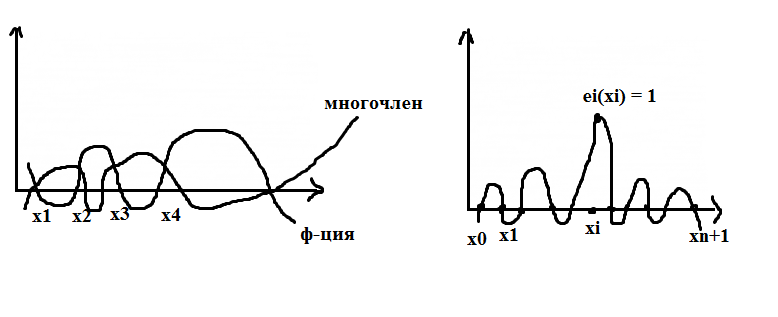
\includegraphics[scale=0.6]{7-1.PNG}
\end{figure}\\
Линейно независимый $\Leftrightarrow$ каждый вектор $v \in V$ представляется в виде $v = x_1 e_1 + ... + x_n e_n$ не более чем одним способом.\\
Упр: (а) любой набор линейно независимых векторов можно дополнить до базиса\\
(b) из любого порождающего набора векторов можно выделить базис.\\
\textit{\textbf{Теорема:}} все базисы в $V$ равномощны. \\
\textit{\textbf{Доказательство:}}\\
Главный инструмент - приведение матрицы к ступенчатому виду.
Пусть $(e_1, ... , e_n), (f_1, ... , f_m)$ два базиса в $V$ ($m \leq n)$\\
Так как $(f_1, ... , f_m)$ - базис, можно выразить $e_i = a_{1i} f_1 + ... + a_{mi} f_m \Leftrightarrow 
e_i = 
\begin{pmatrix}
    a_{1i}\\
    ... \\
    a_{mi}
\end{pmatrix}$ \\
$\begin{pmatrix}
    a_{11} a_{12} ... a_{1n}\\
    ... ... ... ... \\
    a_{m1} a_{m2} ... a_{mn}
\end{pmatrix}$
$\begin{pmatrix}
    x_1 \\
    ... \\
    x_n
\end{pmatrix}$
$=
\begin{pmatrix}
    0 \\
    ... \\
    0
\end{pmatrix}$\\
$x_1 e_1 + x_2 e_2 + ... + x_n e_n = 0$ m линейных уравнений, n неизвестных \\
Так как матрица ступенчтатого вида $\Rightarrow x_2$ может быть любым: $x_2 = 1, x_i$ подберем $\Rightarrow$ получится линейно зависимый \\
$e_1, ... , e_n$ линейно независимы $\Leftrightarrow$ система имеет единственное решение $x_1 = x_2 = ... = x_n = 0.$\\
Если $n > m$ аналогично. \\
$\Rightarrow m = n$. \textbf{ЧТД} \\
\textit{Опр.} \textbf{Размерность пространства} $V$ - количество элементов в базисе $dim V$.\\
\textit{Опр.} \textbf{Линейный оператор} $T: V_1 \rightarrow V_2$ - это отображение, такое что: \\
(1) $T(u + v) = T(u) + T(v)$\\
(2) $T(\lambda v) = \lambda T(v)$.\\
\textit{Опр.} $V_1 \simeq V_2$ (\textbf{изоморфно}) $\Leftrightarrow$ существует взаимно однозначный линейный оператор $T = V_1 \rightarrow V_2$.\\
\textit{\textbf{Теорема:}} любой конечномерное векторное пространство $V$ изоморфно $\mathbb{F}^n (n = dim V)$.\\
\textit{\textbf{Доказательство:}} \\
Выберем базис $(e_1, ... , e_n)$ в $V$\\
$T: v \mapsto (x_1, ... , x_n) \in \mathbb{F}$, где $v = x_1 e_1 + ... + x_n e_n$. \textbf{ЧТД} \\
\textit{Опр.} \textbf{Ядро оператора} $Ker T = \{ v \in V_1 | T(v) = 0 \}$ \\
\textit{Опр.} \textbf{Образ оператора} $Im T = \{ w \in V_2 | w = T(v) \}$ \\

%8 done 
\item \textbf{Определения: матрица линейного оператора, ранг линейного оператора и матрицы. Примеры: движения плоскости, преобразование фоторедактора, дифференцирование многочленов, линейные функции. Как выбрать базисы в области определения и области значений, чтобы матрица линейного оператора имела наиболее простой вид. При композиции линейных операторов их матрицы перемножаются. Ранг оператора равен размерности его области определения минус размерность ядра. Критерии обратимости линейного оператора в терминах его ядра и образа.}\\
Линейные операторы(=линейные отображения = гомоморфизм векторных пространств)\\
Опр: $V\diagup \mathbb{F}, W\diagup \mathbb{F}$ - векторные пространства\\
$T: V \longrightarrow W -$ отображение линейно, если:\\
(1)$T(v+u) = T(v) + T(u)$ для всех $v,u \in V$\\
(2)$T(\lambda v) = \lambda T(V) (\in W)$ для всех $v\in V$\\
Пример: $(1)$ движения плоскости, сохраняющее $O\in \mathbb{R}^2$ \\
(2) $T: (x,y) \longrightarrow (ax, by)$ - линейное отображение, вообще говоря, не движение\\
(3)дифференцирование функции $\mathbb{R} [x] \longrightarrow \mathbb{R} [x], f\longrightarrow f'$\\
(4) $dim W = 1 , W = \mathbb{F}$\\
линейные функции\\
$\phi: V\longrightarrow \mathbb{F}$\\
Например: $\mathbb{R}^2 \longrightarrow \mathbb{R}\\
(x,y) \longrightarrow (ax, by)$\\
\textbf{Свойства умножения матриц:}\\
$1)A(B+C) = AB + AC\\
2) A \lambda = \lambda A\\
X = \begin{pmatrix}
x_1\\
.\\
.\\
.\\
x_n
\end{pmatrix}\\
X' = \begin{pmatrix}
x_1 '\\
.\\
.\\
.\\
x_n '\\
\end{pmatrix}
T_A (X+X') = T_A (X) + T_A(X')$\\
Левая часть - $A\cdot (X+X') = AX + AX' = T_A (X) + T_A (X')$ - правая часть\\
\textbf{Матрица линейного оператора}\\
$e = \{e_1, ..., e_n\} -$ базис в $V$\\
$f = \{ f_1, ..., f_m\} -$ базис в $W$\\
$T: V \longrightarrow W\\
m\times n$ матрица $[T]_{e,f}$\\
$T(e_1) = a_{11} f_1 + a_{21} f_2 + ... + a_{m1} f_m\\
T(e_2) = a_{12} f_1 + a_{22} f_2 + ... + a_{m2} f_m\\
...\\
T(e_nn) = a_{1n} f_1 + a_{2n} f_2 + ... + a_{mn} f_m$\\
Пример: $n =2, m = 3\\
T: V^2 \longrightarrow W^3\\
\{e_1, e_2\}, \{f_1, f_2, f_3\}
V = x_1 e_1 + x_2 e_2\\
\begin{pmatrix}
a_{11} & a_{12}\\
a_{21} & a_{22}\\
a_{31} & a_{32}\\
\end{pmatrix} \begin{pmatrix}
x_1\\
x_2
\end{pmatrix}\\
T(e_1) = a_{11} f_1 + a_{21} f_2 + a_{31} f_3\\
T(e_2) = a_{12} f_1 + a_{22} f_2 + a_{32} f_3\\
T(V) = x_1 \cdot T(e_1) + x_2 T(e_2) = x_1 (a_{11} f_1 + a_{21} f_2 + a_{31} f_3) + x_2 (a_{12} f_1 + a_{22} f_2 + a_{32} f_3) = (x_1 a_{11} + x_2 a_{12}) f_1 + (x_1 a_{21} + x_2 a_{22}) f_2 + (x_1 a_{31} + x_2 a_{32}) f_3 = \begin{pmatrix}
a_{11} x_1 + a_{12} x_2\\
a_{21} x_1 + a_{22} x_2\\
a_{31} x_1 + a_{32} x_2\\
\end{pmatrix}$\\
\textbf{Вопрос: насколько простой может быть матрица $[T]_{e,f}$ для данного $T: V \longrightarrow W$? }\\
Ответ: \begin{figure}[h!]
\centering
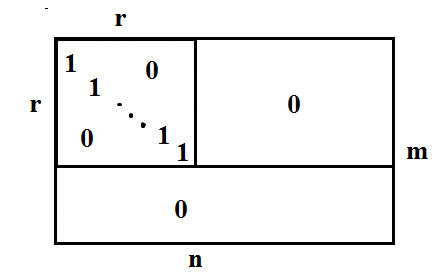
\includegraphics[scale=0.6]{8-1.PNG}
\end{figure}\\
$r \leq  min \{m,n\}$\\
r = ранг оператора T\\
Напоминание: $0 \in Im T \subset W$ - образ $=$ подпространство $\{ W| W = T(v) \}$ для некоторого $v\in V$\\
$Ker T \subset V$ - ядро $= \{v| t(v) = 0\}$\\
\textbf{Опр}: ранг оператора $rk T = dim Im T$\\
$r = m \Longleftrightarrow rk T = dim V$\\
\begin{figure}[h!]
\centering
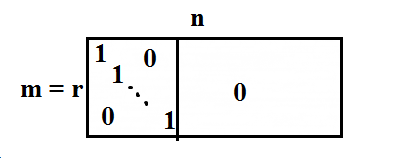
\includegraphics[scale=0.6]{8-2.PNG}
\end{figure}\\
$m = n = r$\\
\begin{figure}[h!]
\centering
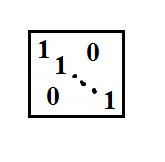
\includegraphics[scale=0.6]{8-3.PNG}
\end{figure}\\
Предложение: $r = rk T$\\
Док-во: $e_1,..,e_n$\\
$f_1,..,f_m$\\
$T(e_1)=f_1,..,T(e_r)=f_r, T(e_k)=0,$ при $k>r$\\
$ImT=<f_1,..,f_r> \Longrightarrow dim(ImT)=r$\\
Предл: Для любого оператора $T: V^n \longrightarrow W^m$ существуют базисы $e_1,..,e_n$ в $V$ и $f_1,..,f_m$ в $W,$ такие что \begin{figure}[h!]
\centering
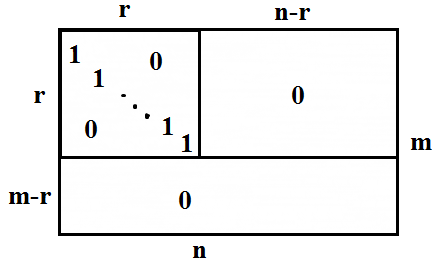
\includegraphics[scale=0.6]{8-4.PNG}
\end{figure}\\
\textbf{Док-во вопроса:} $e^\prime_1,..,e^\prime_n$ - произв. базис в $V$\\
$f^\prime_1,..,f^\prime_m$ - произв. базис в $W$\\
$A={[T]}_{e^\prime f^\prime}$ элементарными преобразованиями строк и столбцов можно привести к виду как на картинке\\
Преобр. строк = замена базиса в $W$\\
Преобр. строк = замена базиса в $V$\\
\textbf{Теорема:} $rkT=dim(V)-dim(KerT), T:V \longrightarrow W$\\
$v_1,..,v_k -$ базис в $V,$ дополним до базиса в $W:v_1,..,v_k,v_{k+1},..,v_n$\\
Лемма: $T(v_{k+1}),..,T(v_n) -$ базис в $ImT$\\
они все порождают, $a_{k+1}T(v_{k+1})+...+a_nT(v_n)=0 \Longrightarrow T(a_{k+1}v_{k+1}+...+a_nv_n)=0 \Longrightarrow (a_{k+1}v_{k+1}+...+a_nv_n) \in KerT \Longrightarrow a_{k+1},..,a_n=0,$ \textbf{чтд!}\\
\textbf{Критерии обратимости линейного оператора в терминах его ядра и образа}\\
Линейный оператор $T: V \longrightarrow W$ обратим $\Longleftrightarrow$ (1) $Ker(A)=0$\\
(2) его матрица $A$ не вырождена $(det(A) \neq 0)$\\
\textbf{Опред:} Линейный оператор $T$ называется обратимым, если $\exists B \in V: AB=BA=I$\\
\textbf{Док-во:} Докажем, что $A$ инъективно, то есть для $\forall a,b \in V: A(a)=A(b) \Longrightarrow a=b$\\
Если $A(a)=A(b),$ то $B(A(a))=B(A(b)) \Longrightarrow (BA)(a)=(BA)(b),$ т.е $I(a)=I(b) \Longrightarrow a=b,$ чтд!\\
(1) Тогда т.к $A$ - инъекция, то нулевой вектор имеет единственный прообраз при отображении $A$, т.е $Ker(A)=0,$ чтд!\\
(2) По построению обратной матрицы как матрицы перехода $A$ к $I,$ и  $Ker(A)=0$ чтд\\

%9 done
\item \textbf{Определения: определитель как ориентированный объем параллелепипеда, определитель линейного оператора, определитель матрицы. Примеры:определители в размерности 2 и 3, равносоставленные параллелограммы имеют равные площади. Вычисление определителя с помощью элементарных преобращований столбцов. Явная формула для определителя.}\\
Опр: $v_1, v_2, ..., v_n \in V^n \diagup \mathbb{F}$ - набор векторов
$det(v_1, v_2, ..., v_n) \in \mathbb{F}$ - объем параллелепипеда, натянутого на векторы $v_1, v_2, ..., v_n (\Pi (v_1, v_2, ..., v_n))$\\
Опр: $T: V^n \longrightarrow V^n$ - линейный оператор\\
$det(T)$ - во столько раз $T$ меняет объем параллелепипеда $\Pi (e_1, e_2, ..., e_n)\\
e_1, e_2, ..., e_n\\
T(e_1), T(e_2), ..., T(e_n)\\
det(T) = \frac{det(T(e_1), T(e_2), ..., T(e_n))}{det(e_1, e_2, e_3, ..., e_n)}$\\
Опр: $A - n \times n$ матрица, $a_{ij} \in \mathbb{F}\\
det A =$ многочлен от $a_{ij}$, такой что:\\
$(1)det A = 0 \Longleftrightarrow rk (A) \textless n\\
(2) det I = 1, I$ - единичная матрица\\
\textbf{Определители в размерности 2 и 3}
$det (\begin{pmatrix}
a & b \\
c & d
\end{pmatrix}) = ad - bc\\
det(\begin{pmatrix}
a_1 & a_2 & a_3\\
b_1 & b_2 & b_3\\
c_1 & c_2 & c_3\\
\end{pmatrix}) = a_1 \cdot b_2 \cdot c_3 + a_2 \cdot b_3 \cdot c_1 + a_3 \cdot b_1 \cdot c_2 - a_3 \cdot b_2 \cdot c_1 - a_1 \cdot b_3 \cdot c_2 - c_3 \cdot a_2 \cdot b_1$ \\
Равносоставленные параллелограммы имеют равные площади, так как они составлены из одинаковых векторов, а значит можно составить две одинаковые матрицы, у которых определители будут равны, а определители размерности 2 - это площадь параллелограммов.\\
\textbf{Элементарные преобразования столбцов}\\
(1)При преобразовании столбцов I типа $(C_i \longrightarrow \lambda C_j + C_i)$ определитель не меняется\\
$det(\begin{pmatrix}
a & b\\
c & d\\
\end{pmatrix})\\
det(\begin{pmatrix}
a+b & b\\
c+d & d\\
\end{pmatrix}) = det(\begin{pmatrix}
a & b\\
c & d\\
\end{pmatrix}) + det(\begin{pmatrix}
b & b\\ 
d & d\\
\end{pmatrix})$ (последний определитель равен 0)\\
(2)При преобразовании столбцов II типа $(C_i \longrightarrow \lambda C_j, \lambda \neq 0)$ определитель умножается на $\lambda\\
det(\begin{pmatrix}
a & \lambda b\\
c & \lambda d\\
\end{pmatrix}) = det(\begin{pmatrix}
a & b\\ 
c & d\\
\end{pmatrix}) \cdot \lambda$\\
(3) При преобразовании столбцов III типа $(C_i \longrightarrow C_j)$ определитель меняет знак\\
$det(\begin{pmatrix}
a & c\\
b & d\\
\end{pmatrix}) = - det (\begin{pmatrix}
c & a\\
d & b\\
\end{pmatrix})$

Явная формула для определителя: \\
Для квадратной матрицы  $A=(a_{ij}) $ размера  $n\times n$  её определитель $\det A$ вычисляется по формуле:

$\det A=\sum _{\alpha _{1},\alpha _{2},\ldots ,\alpha _{n}}(-1)^{N(\alpha _{1},\alpha _{2},\ldots ,\alpha _{n})}\cdot a_{1\alpha _{1}}a_{2\alpha _{2}}\dots a_{n\alpha _{n}}$, где суммирование проводится по всем перестановкам $ \alpha _{1},\alpha _{2},\ldots ,\alpha _{n}$ чисел  $1,2,\dots ,n$, а  $N(\alpha _{1},\alpha _{2},\ldots ,\alpha _{n})  $ обозначает число инверсий в перестановке  $\alpha _{1},\alpha _{2},\ldots ,\alpha _{n}$.
Таким образом, в определитель входит  $n!$ слагаемых, которые также называют «членами определителя».



%10 done
\item \textbf{Определения: аксиоматическое определение определителя(полилинейность, кососимметричность, нормировка); аффинные пространства и подпространства, репер. Примеры: векторное произведение как внешнее; пространство решений неоднородной системы линейных уравнений. Теорема существования и единственности определителя. Разложение определителя по строке. Определитель произведения матриц равен произведению определителей. Связь понятия репера и понятия базиса.}\\

\textbf{Определитель} - функция на наборах из $n$ векторов $v_1, ..., v_n \in V^{n}$ со значениями в $\mathbb{F}$, $det(v_1, ..., v_n) \in V^{n}$ удовлетворяет следующим аксиомам:\\
(1) полилинейность\\
$det(.., v_i+av,..)=det(.., v_i,..)+adet(.., v,..)$\\
(2) кососимметричность\\
$det(.., v_i,..,v_j,..)=-det(..,v_j,..,v_i,..)$\\
(3) $(e_1,..,e_n) -$ эталонный базис в $V^{n}$\\
$det(e_1,..,e_n)=1$\\
\textbf{Теорема} о существовании и единственности определителя\\
\textbf{Док-во:} индукция по $n$\\
1) База: $n=1; V=<e_1>$\\
$v=ae_1$\\
$det(v)=a$\\
$det(ae_1)+det(be_1)=det(ae_1+be_1)=det((a+b)e_1)=a+b$\\
2) Индукционный переход $n \longrightarrow n+1$\\
$V^{n} \subset V^{n+1}$\\
Если $<v_1,..,v_n>$ - подпр-во, натянутое на векторы $v_1,..,v_n$, тогда $V^{n+1}=<e_1,..,e_{n+1}>(det_{n+1}),$ а $V^n=<e_2,..,e_{n+1}>(det_n),$\\
где $det_n(v_2,..,v_{n+1})=det_{n+1}(e_1,v_2,..,v_{n+1})$\\
$v_1=a_{11}e_1+a_{21}e_2+..+a_{(n+1)1}e_{n+1}$\\
$...$\\
$v_{n+1}=a_{1(n+1)}e_1+a_{2(n+1)}e_2+..+a_{(n+1)(n+1)}e_{n+1}$\\
$det_{n+1}(v_1,..,v_{n+1})=det_{n+1}(a_{11}e_1+u_1,..,a_{1(n+1)}e_{n+1}+u_{n+1}),$ где $u_i=v_i-a_{1i}e_1$\\
$det_{n+1}(a_{11}e_1+u_1,..,a_{1(n+1)}e_{n+1}+u_{n+1})=a_{11}det_{n+1}(e_1, v_2,..,v_{n+1})+det_{n+1}(v_1,..,v_{n+1})=a_{11}det_{n+1}(e_1,..,v_{n+1})+a_{12}det_{n+1}(v_1,e_1,..,v_{n+1})+...+a_{1(n+1)}det_{n+1}(v_1,..,e_1)=det_{n+1}(e_1,..,v_{n+1})+a_{12}det_{n+1}(e_1,e_1,v_3,..,v_{n+1}),$ где $a_{12}det_{n+1}(e_1,e_1,v_3,..,v_{n+1})=0$\\
Осталось только вычислить: $det_{n+1}(v_1,v_2,..,v_{i-1},e_1,v_{i+1},..,v_{n+1})=(-1)^{i-1}det_{n+1}(v_1,v_2,..,v_i,..,v_{n+1})=(-1)^{i-1}det_n(v_1,..,\widehat v_i,..,v_{n+1}), \textbf{чтд}$\\
\textbf{Разложение по строке:}\\
$det_{n+1}(v_1,..,v_{n+1})=\sum_{i=1}^{n+1} (-1)^{i-1} \cdot det_n(v_1,..,\widehat v_i,..,v_{n+1})$\\
\textbf{Теорема:} $A, B -$ матрицы $n \times n,$ тогда $det(AB)=det(A) \cdot det(B)$\\
\textbf{Док-во:} $det_n(v_1,..,v_n)=det(A),$ где $v_1,..,v_n -$ столбцы матрицы\\
$\widetilde{det(A)}=det_n(Bv_1,..,Bv_n)$\\
$det(Id)=det_n(Be_1,..,Be_n)=det(B) \Longrightarrow$ (из единственности опр.) $det(A)=$ ${{\widetilde{det(A)}}\over{det(B)}}$ $\Longrightarrow$ $det(A)=$ ${{det(AB)}\over{det(B)}}, \textbf{чтд}$\\
\textbf{Афинное пространство}\\
$\mathbb{A}^n -$ аффинное пр-во над полем $\mathbb{F} -$ векторное пр-во $\mathbb{F}^n,$ в котором нулевой вектор ничем не отличается от остальных\\
\textbf{(1)} любое векторное подпр-во содержит $0$\\
\textbf{(2)} $v \in \mathbb{F}^n, v\neq0,$ неверно, что любое подпр-во содержит $v$\\
\textdf{$\mathbb{A}^n$ как множество совпадает с $\mathbb{F}^n,$ содержащим $0$}\\
\textbf{(3)} $V \subset \mathbb{A}^n -$ аффинное подпр-во, если $V$ паралл. векторному подпр-ву $U \subset \mathbb{F}^n$\\
\textbf{(4)} для каждой пары точек $a,b \in \mathbb{A}^n$ однозначно определен вектор $\overrightarrow{ab} \in \mathbb{F}^n$\\
\textbf{Определение:} Репер в $\mathbb{A}^n$ - точка (нач. коорд.) и базис в $\mathbb{F}^n$\\
\textbf{Пример:} $A$ - матрица $m \times n$\\
$A \cdot X = B$\\
$X=\begin{pmatrix} {x_1}\\
  {...}\\
  {x_n}\\
\end{pmatrix}$\\
$B=\begin{pmatrix} {b_1}\\
  {...}\\
  {b_n}\\
\end{pmatrix}$\\
При $n=2, m=1\\
ax_1+cx_2=b_1=1$\\
$(x_1,x_2), (y_1,y_2) -$ решения, но $((x_1+y_1),(x_2,y_2)) -$ не решения, $\Longrightarrow$ пр-во решений не векторное, а аффинное, оно параллельно векторному пр-ву решений однородной системы $A \cdot X = 0$ $\Longrightarrow$ $V_b=a+V_a, a \in V_b$\\

%11 done 
\item \textbf{Определения: евклидовы пространства, длины, углы, расстояния, ортогональное дополнение к подпространству, ортогональный и ортонормированный базисы. Примеры: школьная плоскость, физическое пространство. Теорема Пифагора. Неравенство треугольника. Расстояние от точки до подпространства, угол между вектором и подпространством, расстояние между скрещивающимися подпространствами.}\\

\textdf{Опред:} Вещественное векторное пр-во $V$ называют \textdf{евклидовым}, если на нем задана положительно определенная билинейная форма $S: (v,u) \Longrightarrow S(v,u) \in \mathbb{R}; v,u \in V,$ причем\\
\textbf{(1)} билинейная: $S(v_1+v_2,u)=S(v_1,u)+S(v_2,u); S(v,u_1+u_2)=S(v,u_1)+S(v,u_2); S(\lambda v,u)=\lambda S(v,u)=S(v,\lambda u)$\\
\textbf{(2)} симметричная: $S(v,u)=S(u,v)$\\
\textbf{(3)} положительно определенная: $S(v,v)=0 \Leftrightarrow v=0$ и $S>0,$ если $v \neq 0$\\
\textbf{Длина вектора:} $|v|_S=\sqrt{S(v,v)}$\\
Афинное пр-во $A$ называется евклидовым, если ассоциированное с ним векторное пр-во $V_A$ - евклидово\\
$d(a,b)=\overrightarrow{ab}$\\
\textbf{Примеры:} (1) Школьная пл-ть\\
$S(v,u)=v_1u_1+v_2u_2$\\
$|v|=\sqrt{{v_1}^2+{v_2}^2}$\\
единичная окр-ть \{$v | |v|=1$\}\\
(2) Физическое пр-во $\mathbb{R}^3$\\
$S(v,u)=v_1u_1+v_2u_2+v_3u_3$\\
$|v|=\sqrt{v^2_1+v^2_2+v^2_3}$\\
$U,W \subset V -$ подпр-ва евкл. пр-ва $V,$ тогда $U \perp W$ (подпр-ва ортогональны или перпендикулярны), если для $\forall u,w \in V (u,w)=0 \Longrightarrow U \cap W=\{0\}$\\
\textbf{Ортогональное дополнение} $U^{\perp}, U \subset V$\\
$U^{\perp}=\{v \in V| (v,u)=0, \forall u \in U\}$\\
$dim(U)+dim(U^{\perp})=dim(V) \Longrightarrow \forall v \in V$ представляется единственным образом как $v=u+u^{\perp}$\\
\textbf{Теорема Пифагора:} $(v,u)=0 \Longrightarrow |\overrightarrow v|^2+|\overrightarrow u|^2=|\overrightarrow v + \overrightarrow u|^2$ (далее будем писать без значка вектора)\\
\textbf{Док-во:} $|u|^2=S(u,u); |v|^2=S(v,v); |v+u|^2=S(v+u,v+u)$\\
$S(v+u,v+u)=S(v,v+u)+S(u,v+u)=S(v,v)+S(v,u)+S(u,v)+S(u,u), S(v,u)=S(u,v)=0 \Longrightarrow$ \textbf{чтд!}\\
\textbf{Расстояние от точки $p \in V$ до подпр-ва $U \subset V$}\\
$d(p,U)=min d(p,q), q \in U$\\
$d(p,q)$ минимально, если $\overrightarrow{pq} \perp U$\\
\textbf{Док-во:} $|\overrightarrow{pq_0}| \perp U; q_0 \in U,$ тогда $\forall q \in U, q \neq q_0: |\overrightarrow{pq}|>|\overrightarrow{pq_0}|,$ \textbf{чтд!}\\
\textbf{Определение угла между вектором и подпр-вом}\\
$U \subset \mathbb{A}, v \in V, U -$ подпр-во\\
$cos(v,u)=cos(min(v,u)), |u|=1, u \in U$\\
$v=u_0+u^{\perp}_0, u^{\perp}_0 \in U$\\
$cos(v,u)={(v,u) \over{\sqrt{v^2_1+v^2_2} \sqrt{u^2_1+u^2_2}}}$\\
$cos(v,u_0)>cos(v,u)$ \\
\begin{figure}[h!]
\centering
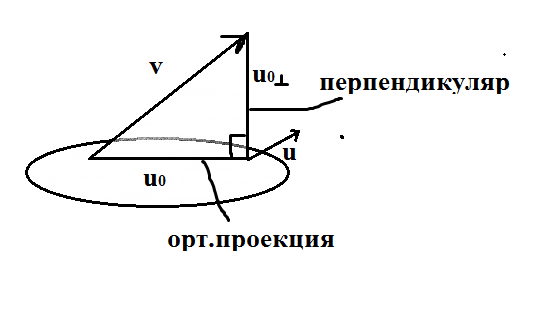
\includegraphics[scale=0.6]{11-1.PNG}
\end{figure}\\
$v=u_0+u^{\perp}_0, (v,u)=(u_0+u^{\perp}_0, u)=(u_0,u)+(u^{\perp}_0,u)=(u_0,u) \Longrightarrow$ максимум достигается, когда $u=\lambda u_0$\\
\textbf{Ортонормированный базис} $\overrightarrow e_1,..,\overrightarrow e_n - $ это базис, в котором все векторы попарно ортогональны и $(e_i,e_j)=0, i \neq j; (e_i,e_j)=1, i=j$\\
\textbf{Расстояние между скрещивающимися подпр-ми}\\
$U,W \subset \mathbb{A}, dim(W)\geq dim(U)$\\
$U,W -$ скрещиваются, если $U \cap W=\varnothing$ и $U$ не параллельно $W$ (не сущ-ет парал. переноса, переводящего одно в другое)\\
$d(U,W)=mind(p,q), p \in U, q \in W,$ минимум реализуется, когда $\overrightarrow{pq} \perp U,W$\\

%12 АРТЕМ 
\item \textbf{Определения: матрица Грама билинейной формы. Примеры: матрица Грама стандартного скалярного произведения. Ортогонализация Грама-Шмидта для положительно определенной симметричной билинейной формы. Квадрат объема параллелепипеда как определитель матрицы Грама. Неравенство Коши-Буняковского-Шварца. Формула для расстояние от вектора до подпространства через матрицы Грама. Разложение вектора по ортонормальному базису. Метод наименьших квадратов.}\\
\textbf{Определения: матрица Грама билинейной формы} $ s(\cdot,\cdot)$ на $\bb{R}^n$ в базисе $e_1, e_2,..,e_n$ - это $n\times n$ матрица\\
$A_s=\begin{pmatrix}
s(e_1,e_1) & s(e_1,e_2) & ... & s(e_1,e_n)\\
s(e_2,e_1) & s(e_2,e_2) & ... & s(e_2,e_n)\\
... & ... & ... & ...\\
s(e_n,e_1) & s(e_n,e_2) & ... & s(e_n,e_n)\\
\end{pmatrix}$, где $s(e_1,e_2) = s(e_2,e_1)$ и т.п.\\
$(u_1, .., u_n)\cdot A_s \cdot \begin{pmatrix}
v_1\\
v_2\\
v_3\\
\end{pmatrix}=s(u,v)$\\
Пример: матрица Грама стандартного скалярного произведения $s(u,v)=\sum_{i=1} u_iv_i, \  s(v,v)=\sum_{i=1}^{n} v_i^2 >0$ \  при $v\neq 0$\\
$A_s=\begin{pmatrix}
1 & ... & ... & 0\\
0 & 1 & ... & 0\\
... & ... & ... & ...\\
0 & ... & 0 & 1\\
\end{pmatrix} s(e_i,e_i)=1, s(e_i,e_J)=0 \ (i\neq j)$\\
\textbf{Ортогонализация Грама-Шмидта для положительно определенной симметричной билинейной формы}\\
Теорема: каждая полож. опред. симметричная билинейная форма $s(\cdot,\cdot)$ на $\bb{R}^{n}$ в некотором базисе имеет единичную матрицу Грама.\\
Более того, этот базис $(v_1, ..., v_n)$ получился из данного $(e_1, ..., e_n)$ верхнетреуг. преобразованиями, т.е.\\
$v_1 = a_{11} \cdot e_1\\
v_2==a_{12}\cdot e_1 +a_{22}\cdot e_2\\
v_n=a_{1n}\cdot e_1 +...+a_{nn} \cdot e_n$.\\
Опр: $(v_1,... ,v_n)$ ортонормальный базис $\Longleftrightarrow A_s = \begin{pmatrix}
1 & ... & ... & 0\\
0 & 1 & ... & 0\\
... & ... & ... & ...\\
0 & ... & 0 & 1\\
\end{pmatrix}$ в этом базисе. \\
Док-во:\\
$|v_1|=|v_2|=1 \ v_1=a_{11}\cdot e_1, \ v_2=a_{12}\cdot e_1 + a_{22}\cdot e_2 \Rightarrow$ просто подбираем $a_{11}$ таким чтоб $v_1$ был единичной длинны. $a_{11}=\frac{1}{\sqrt{(e_1,e_1)}}$\\
\begin{figure}[h!]
\centering
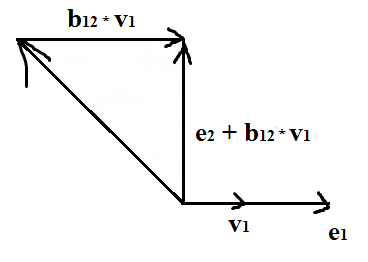
\includegraphics[scale=0.6]{12-1.PNG}
\end{figure}\\
Доказываем индукцией по n. для n=1 доказали.\\
Шаг индукции. (n-1) доказано $\Rightarrow$ докажем для n.\\
Подберем $b_{12}$ так что $(e_2 + b_{12}\cdot v_1, v_1)=0\\
(e_2, v_1)+b_{12}\cdot (v_1,v_1) \Rightarrow b_{12}= - (e_2, v_1)$ точно так же находим $b_{ij}=(e_i, v_1)$ Заменим $e_i$ на $\widetilde{e_i} =e_i -(e_i,v_1)\cdot v_1$ Получим базис $v_1, \widetilde{e_2} , ..., \widetilde{e_n}$ . применим предположение индукции для $\widetilde{e_i}$\\
\textbf{Неравенство Коши-Буняковского-Шварца}\\
$|\cos{\phi}|= |\frac{(u,v)}{\sqrt{(u,u)(v,v)}}|\leq 1\\
{(u,v)}^2 \leq (u,u)(v,v)$ для $\forall u,v \in \bb(R)^n$\\
$detA=(u,u)(v,v)-{(u,v)}^2$ где А это матрица Грама. Ее определитель всегда $\geq 0$\\
$|vol(n(v_1, ..., v_n))|=|detC|=\sqrt{detA}$ где С это матрица для которой верно $(v_1, ..., v_n)=(e_1, ..., e_n)C$, а А это матрица Грама в базисе $v_1, .., v_n$\\
<$u_1, ..., u_k> \in \bb{R}^n$ - подпространство. \  $\stackrel{\rightarrow}{op}=v \in \bb{R}^n \ d(p,U)\cdot \sqrt{detA(u_1,...,u_k)}=\sqrt{detA(u_1, ..., u_k, v)} \Rightarrow d(p,U)^2=\frac{detA(u_1, ..., u_k, v)}{detA(u_1, ..., u_k)} \\
u_1, ..., u_k$ -ортонормальный набор векторов. $v=(v,u_1)u_1 + (v,u_2)u_2 + ... + (v,u_k)u_k$, где ($(v,u_k)u_k=pr_nv$) \ разложение по $u_1, ..., u_k$, если $v \in U$, если нет, то наилучшее приближение $\min|v-v_0|=|v-pr_nv|$ где $v_0 \in U$

%13 Зимина (изометрия - линейное преобразование)
\item \textbf{Определения: изометрии(движения) евклидова пространства, группы $GL_n (\bb{R})$ (полная линейна), $SL_n (\bb{R})$ (специальная линейная), $O_n(\bb{R})$ (ортогональная), $SO_n(\bb{R})$ (специальная ортогональная). Примеры: группа $O_2(\bb{R})$, группа поворотов плоскости $SO_2(\bb{R})$, группа поворотов трехмерного пространства $SO_3(\bb{R})$. Изометрия является линейным преобразованием. Классификация движения плоскости.}\\

\textit{Опр.} \textbf{Евклидово пространство} - конечномерное вещественное векторное пространство $\mathbb{R}^n$ с ведённым на них положительно определенным скалярным произведением, либо метрическое пространство, соответствующее такому векторному пространству. \\
\textit{Опр.} Отображение $T: \mathbb{R}^n \rightarrow \mathbb{R}^n$ - \textbf{изометрия (= движение)}, если $d(T(a), T(b)) = d(a, b)$ для любых $a, b \in \mathbb{R}^n$ (d - расстояние).\\
\textit{Опр.} \textbf{$O_n(\mathbb{R})$ ортогональная группа} - группа изометрий векторного пространства.\\
\textit{Опр.} \textbf{$SO_n(\mathbb{R})$ специальная ортогональная группа} - группа вещественных ортогональных матриц размера $n \times n$ с определителем, равным 1. \\
\textit{Опр.} \textbf{$GL_n(\mathbb{R}$) полная линейная группа} - группа всех обратимых линейных операторов в $\mathbb{R}^n$ \\
\textit{Опр.} \textbf{$SL_n(\mathbb{R}$ специальная линейная группа} = $\{ A \in GL_n(\mathbb{R}) | det A = 1 \}$\\
$O_n(\mathbb{R}) \subset GL_n(\mathbb{R})$; $SL_n(\mathbb{R}) \subset GL_n(\mathbb{R})$ \\
Примеры: \\
(1) группа $O_2(\bb{R})$ \\
Это композиция поворота и отражения 
\\
Матрица поворота
$\begin{pmatrix}
     \cos{\phi} \ -\sin{\phi}\\
     \sin{\phi} \ \cos{\phi} 
\end{pmatrix} \\$
Матрица отражения относительно прямой $y = kx + b$
$\begin{pmatrix}
    2\frac{1 - kb}{k^2 + 1}-1 \ \ 2\frac{k - kb}{k^2 + 1} \\
    2k\frac{1 - kb}{k^2 + 1}+2b \ \ 2k\frac{k - kb}{k^2 +1}+2b-1
\end{pmatrix}$ \\
Дальше надо найти композицию этих двух матриц
\\(2) группа поворотов плоскости $SO_2(\bb{R})$ 
Матрица поворота
$\begin{pmatrix}
     \cos{\phi} \ -\sin{\phi}\\
     \sin{\phi} \ \cos{\phi} 
\end{pmatrix} \\$
(3) группа поворотов трехмерного пространства $SO_3(\bb{R})$ 
повороты
$\begin{pmatrix}
    1 \ \ \ \ 0 \ \ \ \ 0 \\
    0 \ \cos{\phi} \ -\sin{\phi} \\
    0 \ \ \sin{\phi} \ \cos{\phi}
\end{pmatrix} \\ $
\textit{\textbf{Изометрия является линейным преобразованием}}\\
Линейное преобразование $T$:\\
1) $T(u + v) = T(u) + T(v)$\\
2) $T(\lambda v) = \lambda T(v)$


\textit{\textbf{Классификация движения плоскости}}\\
\textit{Опр.} Движение, являющееся композицией четного числа симметрий относительно прямых, называют \textbf{движением первого рода} или движением, сохраняющим ориентацию плоскости. \\
\textit{Опр.} Движение, являющееся композицией нечетного числа симметрий относительно прямых, называют \textbf{движением второго рода} или движением, изменяющим ориентацию плоскости. \\
\textit{\textbf{Теорема Шаля.}} Каждое движение первого рода является либо параллельным переносом, либо поворотом; каждое движение второго рода - либо осевая симметрия, либо скользящая симметрия. \\
\textbf{Лемма о трех гвоздях.} Любое движение однозначно задается тремя не лежащими на одной прямой точками и их образами. (Для любых не лежащих на одной прямой точек $A, B, C$ и их образов $A', B', C'$ существует единственное движение $f: A \mapsto A', B \mapsto B', C \mapsto C'$)\\
\textbf{Док-во леммы:}\\
Возьмем любую точку $D \neq A, B, C$, и ее образ $D'.$ $f -$ движение, а значит $AD = A'D' \Rightarrow D'$ лежит на окружности с центром $A'$ и радиусом $AD$. \\
Аналогично для точек $B, C \Rightarrow D'$ также лежит на окружности с центром $B'$ и радиусом $BD$ и на окружности с центром $C'$ и радиусом $CD$. \\
Так как три окружности могут пересекаться только в одной точке, то существует единственный образ $D'$ для любой точки $D$. Это равносильно единственности движения. \textbf{ЧТД} \\
\textbf{Лемма о трех симметриях.} Любое движение представимо в виде композиции не более чем трех осевых симметрий. (Любое движение $f$ представимо или как $S_l$ или как $S_{l_1} \circ S_{l_2},$ или как $S_{l_1} \circ S_{l_2} \circ S_{l_3}.$\\
\textbf{Док-во леммы:}\\
Возьмём любое движение $f$ и точки $A, B, C$ с их образами $A', B', C'.$ Если докажем, что для $A, B, C$ существует композиция симметрий $g$ эквивалентная $f$, то по лемме о трех гвоздях $f = g$ в общем случае. \\
Заметим что $S_{l_i} \circ ... \circ S_{l_1} \circ f = id \Leftrightarrow f = S_{l_1} \circ ... \circ S_{l_i},$ так как $S^{-1}_l$ по определению $= S_l$ и $(f \circ g)^{-1}$ по определению $= g^{-1} \circ f^{-1}.$\\
Найдем представление $f$ в виде композиции осевых симметрий: \\
(1) Рассмотрим симметрию $S_{l_1},$ такую что $A \mapsto A'.$ Точка $B$ при такой симметрии перейдет или в некоторую новую точку $B'_1$, или обратно в $B'$. Точка $C$ аналогично. Если $B, C$ вернулись в $B', C'$, то $S_{l_1} \circ f = id.$ В таком случае $S_{l_1} = f$. \\
(2) Если точка $B \mapsto B'_1,$ то рассмотрим симметрию $S_{l_2},$ такую что $B'_1 \mapsto B'.$ Заметим, что $l_2$ - серединный перпендикуляр к отрезку $B' B'_1$, по определению осевой симметрии. \\
$f, S_{l_1}$ - движения, а значит $AB \overset{f}{=} A'B' \overset{S_{l_1}}{=} A'B'_1.$ Следовательно, $A'$ лежит на серединном перпендикуляре к отрезку $B'B'_1$ (по свойству серединного перпендикуляра), то есть на прямой $l_2$. Отсюда следует, что при преобразовании $S_{l_2} A' \mapsto A'.$ Если $C' \mapsto C,$ то аналогично $CB \overset{f}{=} C'B' \overset{S_{l_1}}{=} CB'_1,$ то есть при $S_{l_2} C$ перейдет в $C'.$ Иначе $C \mapsto C'_1$ значит $C'$ снова перейдет или в некоторую $C'_2$ или в $C'.$ Итого, если или $C'_1 \mapsto C'$ при $S_{l_2};$ или $C \mapsto C'$ при $S_{l_1},$ то $S_{l_2} \circ S_{l_1} \circ f = id.$ Это значит, что $f = S_{l_1} \circ S_{l_2}.$ \\
(3) Если $C \mapsto C'_1 \mapsto C'_2,$ рассмотрим симметрию $S_{l_3},$ такую что $C'_2 \mapsto C'.$\\
Очевидно, что $l_3$ - серединный перпендикуляр к отрезку $C' C'_2. f, S_{l_1}, S_{l_2}$ - движения, а значит $AC \overset{f}{=} A'C' \overset{S_{l_1}}{=} A'C'_1 \overset{S_{l_2}}{=} A'C'_2.$\\
Следовательно, $A'$ принадлежит серединному перпендикуляру к отрезку $C'C'_2,$ то есть $l_3$. Это значит, что $S_{l_3}$ переводит $A'$ в $A'.$ Если $B \mapsto B',$ то аналогично $B' \in l_3.$ Иначе, $B \mapsto B'_1 \mapsto B',$ следовательно $BC \overset{f}{=} B'C' \overset{S_{l_1}}{=} B'_1C'_1 \overset{S_{l_2}}{=} B'C'_2$ и $B'$ тоже лежит на $l_3$. Это значит, что $S_{l_3}$ переводит $B'$ в $B'.$ Следовательно, $S_{l_3} \circ S_{l_2} \circ S_{l_1} \circ f = id,$ а значит, $f = S_{l_1} \circ S_{l_2} \circ S_{l_3}.$ \textbf{ЧТД}\\
\textit{\textbf{Док-во теоремы Шаля:}}\\
Каждое данное движение $f$ представим в виде композиции не более трех симметрий по лемме о трех симметриях. \\
Классифицируем получившееся равенство, тем самым классифицировав любое данное движение:\\
1. Если $f = S_{l_1},$ то $f$ - осевая симметрия.\\
2. Если $f = S_{l_1} \circ S_{l_2},$ то либо $l_1 || l_2$ и $f$ - параллельный перенос, либо $l_1$ не параллельно $l_2$ и тогда $f$ - поворот.\\
3. Иначе, $f = S_{l_1} \circ S_{l_2} \circ S_{l_3}$ и тогда $f$ - скользящая симметрия (по свойству скользящей симметрии). \textbf{ЧТД} \\



%14 done 
\item \textbf{Определения: построение циркулем и линейкой, построимые комплексные числа, расширения полей, поликвадратичные расширения, степень расширения. Примеры: классические задачи древности, построение правильного пятиугольника. Степень башни расширений полей. Доказательство неразрешимости задач об удвоении куба и трисекции угла.}\\
Построения циркулем и линейкой:\\
- даны точки\\
- можно провести через точки прямую\\
- можно построить окружность\\
- найти точку пересечения прямых\\
- найти 2 точки пересечения двух окуржностей\\
- найти точки пересечения окружностей и прямой\\
\textit{Опр.} \textbf{Число $\alpha \in {C}$ - построено}, если существует башня расширений ${K_0} = {\mathbb{Q}_0} \subset {K_1} \subset ... \subset {K_n}$, такая что $\alpha \in {K_n}$\\
\textit{Опр.} \textbf{Расширение поля} $K$ - поле $E$, содержащее данное поле $K$ в качестве подполя\\
\textit{Опр.} $K$ - \textbf{поликвадратичное расширение поля} $\mathbb{Q}$ \Leftrightarrow $\exists$ башня расширений\\
\textit{Опр.} ${K} \subset {E}$. Размерность векторного пространства {E} над {K} называется \textbf{степенью расширения} и обозначается $\textbf{[{E}:{K}]}$\\
$[{E}:{K}]$ = ${dim_K}$E - степень расширения\\
\textit{Пример.} Классические задачи древности: умеем строить биссектрису угла, перпендикуляр, правильный треугольник, квадрат, пятиугольник, шестиугольник\\
\textit{Пример.} Построение правильного пятиугольника\\
1) В первую очередь необходимо построить циркулем окружность. Центр окружности пусть совпадает с точкой O. Проведите оси симметрии перпендикулярные друг другу. В точке пересечения одной из этих осей с окружностью поставьте точку V. Эта точка будет вершиной будущего пятиугольника. В точке пересечения другой оси с окружностью расположите точку D.\\
2) На отрезке OD найдите середину и отметьте в ней точку А. После этого нужно построить циркулем окружность с центром в этой точке. Кроме того, она должна проходить через точку V, то есть, радиусом CV. Точку пересечения оси симметрии и этой окружности обозначьте за В.\\
3) После этого при помощи циркуля проведите окружность такого же радиуса, поставив иголку в точку V. Пересечение этой окружности с первоначальной обозначьте как точку F. Эта точка станет второй вершиной будущего правильного пятиугольника.\\
4) Теперь нужно провести такую же окружность через точку Е, но с центром в F. Пересечение только что проведенной окружности с первоначальной обозначьте как точку G. Эта точка так же станет еще одной из вершин пятиугольника. Аналогичным образом необходимо построить еще один круг. Центр его в G. Точка пересечения его с первоначальной окружностью пусть будет H. Это последняя вершина правильного многоугольника.\\
5) У вас должно получиться пять вершин. Остается их просто соединить по линейке. В результате всех этих операций вы получите вписанный в окружность правильный пятиугольник.\\
\begin{figure}[h!]
\centering
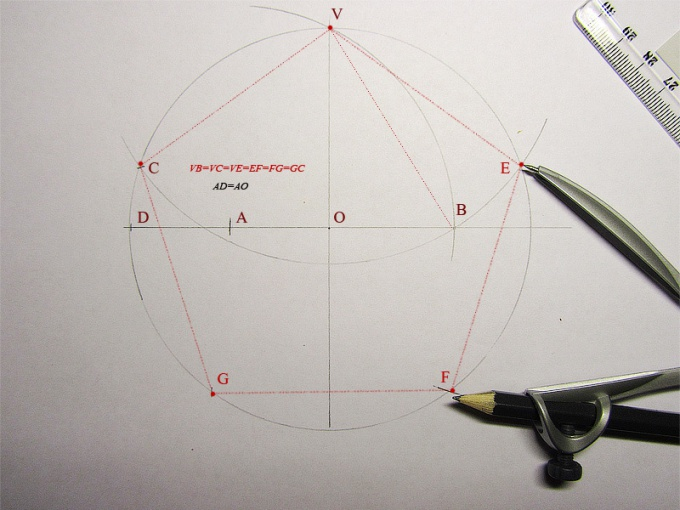
\includegraphics[scale=0.6]{14-1.PNG}
\end{figure}\\
\textbf{Степень башни расширений полей}\\
{K} \subset {F} \subset {E}\\
$[{F}:{K}] \circ [{E}:{F}] = [{E}:{K}]$\\
\textit{Доказательство.} ${\alpha_1},{\alpha_2},...,{\alpha_k}$ - базис векторного пространства {F} над {K}. ${\beta_1},{\beta_2},...,{\beta_l}$ - базис {E} над {F}.\\
$\Rightarrow \{{\alpha_i},{\beta_j}\}$ - базис в {E} над {K} (1 \leq i \leq k; 1 \leq j \leq l)\\
x \in {E}\\
$x = {\lambda_1}{\beta_1} + ... + {\lambda_l}{\beta_l}$, ${\lambda_i} \in {F}$\\
${\lambda_i} = {\mu_1}{\alpha_1} + ... + {\mu_k}{\alpha_k}$, ${\mu_j} \in {K}$\\
\textbf{док-во того, что $\sqrt[3]{2}$ нельзя построить}\\
$\mathbb{K} \subset \mathbb{F}, \mathbb{F}$ - векторное пространство над $\mathbb{K}$\\
$[\mathbb{F}: \mathbb{K}] = dim_k \mathbb{F}$ - степень расширения \\
Док-во: $\mathbb{Q} = \mathbb{K}, \mathbb{F} = \mathbb{Q} (\sqrt{2}) = \{a + b\cdot \sqrt{2} | a,b \in \mathbb{Q} \} \ni \frac{1}{a+b\cdot \sqrt{2}} = \frac{a-b\cdot \sqrt{2}}{a^2 - 2b^2}$\\
$[\mathbb{F}: \mathbb{K}] = 2$\\
Есть базис: $\{1,\sqrt{2}\}$\\
Так не бывает: $p+q\sqrt{2} = 0 \Longrightarrow \sqrt{2} = -\frac{p}{q} \in \mathbb{Q}$ чтд\\
\textbf{Невозможность удвоения куба:}\\
Если данный куб имеет ребро, равное единице, его объем будет равен кубической единице; требуется найти ребро х куба, объем которого вдвое больше. Итак, искомое ребро удовлетворяет простому кубическому уравнению: $x^3 - 2 = 0 \Longrightarrow x = \sqrt[3]{2}$ - что невозможно построить с помощью циркуля и линейки\\
\textbf{Нерешимость задачи про трисекции угла}
Обозначу данный угол, который нужно разделить на три равные части, через $3\alpha$. Рассмотрю $cos 3\alpha$.\\
По известным формулам тригонометрии буду иметь:
$cos 3\alpha = 4cos^3 \alpha - 3cos \alpha$\\
Умножая левую и правую части уравнения на 2, получу , $2cos 3\alpha = 8cos^3 \alpha - 6cos\alpha$. Пусть теперь $2cos 3\alpha = a$, а $2cos \alpha =x$, тогда $a = x^3 - 3x$\\
$x^3 - 3x - a =0$\\
Когда это уравнение для некоторого а разрешимо в квадратных радикалах, то трисекция соответствующего угла выполнима при помощи циркуля и линейки, и наоборот: если для данного угла выполнима трисекция, то соответствующее уравнение должно быть разрешимо в квадратных радикалах.\\
Чтобы доказать, что трисекция угла не разрешима в общем виде, достаточно указать хотя бы один угол, который нельзя разделить при помощи линейки и циркуля на три равные части. Предположим, что $3\alpha=60$, тогда $cos 3\alpha=0.5$, и уравнение примет вид:\\
$x^3 - 3x - 1 = 0$, не разрешимо в квадратных радикалах => нет трисекции чтд


%15 done
\item \textbf{Определения: собственные векторы, собственные значения и характеристический многочлен оператора. Собственные векторы с попарно различными собственными значениями линейно независимы.}\\
Опр: $v$ - собственный вектор оператора $T$  с собственным значением $\lambda$, если $T(v) = \lambda v$\\
Опр': $v\in V$ - собственный вектор оператора $T$ с собственным значением $\lambda$, если $v\in Ker(T - \lambda I)$ (эквивалентное определение)
$Ker(T - \lambda I) \neq \{0\} \Longleftrightarrow rk(T-\lambda I) \textless dim V \Longleftrightarrow det(T - \lambda I) \neq 0$ \\
Пример: $T - \lambda I = \begin{pmatrix}
3 - \lambda & 2\\
1 & 4-\lambda\\
\end{pmatrix} \Longrightarrow det(T - \lambda I) = (3-\lambda)(4-\lambda) - 2 \Longrightarrow det(T - \lambda I) = 12 - 3\lambda - 4\lambda + {\lambda}^2 - 2 \Longrightarrow det(T - \lambda I) = {\lambda}^2 - 7\lambda + 10 \Longrightarrow {\lambda}^2 - 7\lambda + 10 = 0 \Longrightarrow {\lambda}_1 = 2, {\lambda}_2 = 5$\\
Опр: многочлен $det(T - \lambda I)$ называется характеристическим многочленом оператора $T$\\
Предложение: собственное значение = корни характеристического многочлена\\
Док-во: A матрица оператора $T$ \\
$A - \lambda I = \begin{pmatrix}
\\
\\
\\
\\
\\
\\
\end{pmatrix} \cdot \begin{pmatrix}
 x_1\\
 x_2\\
 .\\
 .\\
 .\\
 x_n\\
\end{pmatrix}\\
(A-\lambda I) v = 0$\\
Система имеет ненулевое решение $\Longleftrightarrow det(A-\lambda I) = 0$ \\
Пример: $\lambda = 5, v = \begin{pmatrix}
 x\\
 y\\
\end{pmatrix}\\
\begin{pmatrix}
 3 - 5 & 2\\
 1 & 4 - 5 
\end{pmatrix} \cdot \begin{pmatrix}
 x\\
 y\\
\end{pmatrix} = 0 \\
\begin{pmatrix}
-2 & 2\\
 1 & -1
\end{pmatrix} \cdot \begin{pmatrix}
 x\\
 y\\
\end{pmatrix} = 0 \\
\begin{pmatrix}
  -2x + 2y\\
  x-y
\end{pmatrix} = 0 \Longrightarrow \begin{cases}
-2x + 2y = 0  \\
x - y = 0
\end{cases} \Longrightarrow x = y \Longrightarrow v = \begin{pmatrix}
 1\\
 1\\
\end{pmatrix}$\\
Лемма: $v_1 \neq 0, v_2 \neq 0$ - собственные вектора с собственными значениями ${\lambda}_1 и {\lambda}_2, {\lambda}_1 \neq {\lambda}_2 \Longrightarrow v_1 \neq k v_2, k\in \mathbb{F}$\\
Дано: $T(v_1) = {\lambda}_1 v_1 \\
T(v_2) = {\lambda}_2 v_2\\
v_1 = k v_2 -?$\\
Док-во: пусть да, $v_1 = k v_2 \Longrightarrow T(v_1) = T(kv_2) \Longrightarrow T(v_1) = k T(v_2) \Longrightarrow {\lambda}_1 v_1 = k {\lambda}_2 v_2 \Longrightarrow {\lambda}_1 k v_2 = k {\lambda}_2 v_2 \Longrightarrow ({\lambda}_1 - {\lambda}_2) v_2 = 0 \Longrightarrow$ либо $v_2 = 0$ (противоречит условию), либо ${\lambda}_1 = {\lambda}_2$ (что тоже противоречит условию) чтд

%16 done 
\item \textbf{Определения: диагонализуемые операторы, след оператора, сопряженные (подобные) матрицы. Матрицы оператора в разных базисах сопряжены. Почти любой оператор над полем комплексных чисел диагонализуем. Теорема Гамильтона-Кэли. Вычисление степени оператора с помощью интерполяционного многочлена Лагранжа.}\\
\textnormal $T: V \rightarrow V, dimV=n$\\
\textit{Опр.} \textbf{Характеристический многочлен} $\chi_{T}(\lambda)=det(T- \lambda I)=(-1)^n \lambda^n+...$\\
\textit{Опр.} \textbf{$T$ диагонализуем} $\Leftrightarrow$ все корни характеристического многочлена \ различны $\Leftrightarrow$ есть базис, в котором матрица оператора имеет вид:
\\
$\begin{pmatrix}
  \lambda_{1} & 0 & \ldots & 0\\
  0 & \lambda_{2} & \ldots & 0\\
  \vdots & \vdots & \ddots & 0\\
  0 & 0 & 0 & \lambda_{n}
\end{pmatrix} = 0 = \mathbf{diag(\lambda_{1}, ... , \lambda_{n})}$\\
\textit{Опр.} \textbf{След} оператора $trT= \sum_{i=1}^n a_{ii}$ \\
\textit{Опр.} \exists $ невырожденная матрица $ P $ (квадратная, определитель которой отличен от нуля) $: $ A=PBP^{-1}$ $\Leftrightarrow$ A и В - \textbf{сопряженные}.
\textsl \\
\\\textbf{Матрицы оператора в разных базисах сопряжены}\\
Матрицы $A_b$ и $A_e$  линейного оператора $А: L \rightarrow L$,
записанные в базисах $b$ и $е$ линейного пространства $L$, связаны друг с другом соотношением
$A_{e}=U^{-1}A_{b}U$, где где $U = U_{b \rightarrow e}$ - матрица перехода от базиса $b$ к базису $е$.

Доказательство:
Пусть $y=Ax$. Обозначим координаты векторов х и у в старом базисе b через $x_b$ и $y_b$, а в новом базисе е – через $x_e$ и $y_e$. Поскольку действие линейного оператора А в матричной форме в базисе b имеет вид $y_b = A_b*x_b$ (см. теорему 1), 
а координаты векторов х и у в новом и старом базисах связаны между собой равенствами
$X_b = Ux_e, y_b = Uy_e$,
то получаем
$y_e = U^{-1}_b= U^{-1}(A_bx_b) = U^{-1}(A_bUx_e) = (U{-1}A_bU)х_e$ .
Равенство $y_e = (U^{-1}A_bU) x_e$ является матричной формой записи действия линейного оператора А в базисе е и поэтому, согласно теореме 4.4, $U^{-1}A_bU = A_e$.
Изложенное доказательство теоремы хорошо иллюстрирует следующая диаграмма:
\begin{figure}[h!]
\centering
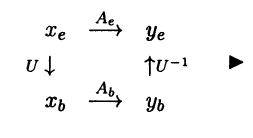
\includegraphics[scale=0.8]{16-1.PNG}
\end{figure}\\
\\
Теорема 1
Пусть $A: L \rightarrow L$ - линейный оператор. Тогда столбец у координат вектора $y=Ax$ в данном базисе b линейного пространства L равен произведению Ах матрицы А оператора А в базисе b на столбец х координат вектора x в том же базисе: $y=Ax$.\\
Доказательство:\\
Выберем произвольный вектор $x = x_1b_1 + … x_nb_n$\\
Его образом будет вектор \\
$y=Ax=A(x_1b_1 + … + x_nb_n) = x_1(Ab_1) + … + x_n(Ab_n) = x_1(a_{11}b_1 + … + a_{n1}b_n) + … + x_n(a_{1n}b_1 + … + a_{nn}b_n) = (a_{11}x_1 + … + a_{1n}x_n)b_1 + … + (a_{n1}x_1 + … + a_{nn}x_{n})b_n$.\\
Столбец координат вектора $Ax$ в базисе $b$ имеет вид\\
\begin{figure}[h!]
\centering
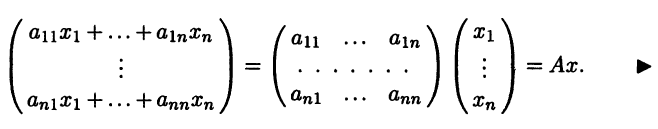
\includegraphics[scale=0.6]{16-2.PNG}
\end{figure}\\

Теорема 2
Пусть b - произвольный базис в n-мерном линейном пространстве L. Различным линейным операторам А и В, действующим в пространстве L, соответствуют и различные матрицы в базисе b. Любая квадратная матрица А порядка n является матрицей некоторого линейного оператора, действующего в линейном пространстве L.\\
Доказательство:\\
Если матрицы А и В операторов А и В в базисе b совпадают, то, согласно теореме 1, для любого вектора х со столбцом координат х\\
$Ax=bAx=bBx=Bx$, т.е. образы произвольного вектора при двух отображениях совпадают. Следовательно, совпадают и сами отображения.\\
Пусть $A=(a_{ij})$ - произвольная квадратная матрица порядка n. Определим отображение $A: L \rightarrow L$ согласно формуле $A(x)=bAx$, где x  - столбец координат вектора х. Несложно проверить, что заданное таким образом отображение является линейным оператором. Действительно, для любых векторов x,y \in L и любых действительных чисел $\lambda$ и $\mu$ \\
$A(\lambda x + \mu у) = bA(\lambda x + \mu y) = \lambda (bAx) + \mu (bAу) = \lambda A(x) + \mu A(y)$.\\
Вычисляем столбец координат образа  i-го вектора из базиса b, где единица стоит в i-й строке, убеждаемся, что он совпадает с i-м столбцом матрицы А и поэтому матрица заданного линейного оператора совпадает с исходной матрицей А. 

\begin{figure}[h!]
\centering
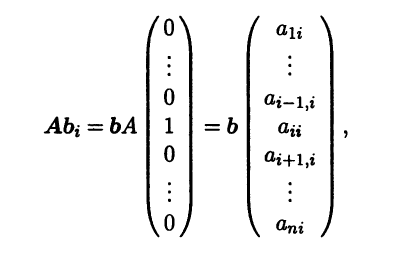
\includegraphics[scale=0.6]{16-3.PNG}
\end{figure}\\

\textbf{Теорема:} Диагонализуемые операторы образуют открытое и всюду плотное множество в пространстве всех операторов $\mathbb{C}^n$.\\
Доказательство:
$n=2$
$A=$
\begin{pmatrix}
  a & b\\
  c & d
\end{pmatrix}\\
$\chi_{T}(\lambda)=\lambda^2-(a+d)\lambda+(ad-bc)$\\
$\chi_{T}(\lambda)$ не имеет кратных решений \Rightarrow A диагонализуем\\
$\lambda^2+p\lambda+q$ имеет кратный корень $\Leftrightarrow$  $p^2-4q=0$, $(a+d)^2=4(ad-bc)=0$ \Leftrightarrow$\\
$\chi_{T}(\lambda)$ не имеет кратные корни\\
\{диагональные операторы\} $ \subset$ \{Операторы T такие, что $\chi_{T}(\lambda)$ не имеет корней\} = \{все операторы\} \setminus \{$D=0$\}\\
\lambda^n+a_1\lambda^{n-1}+...+a_n не имеет кратных корней $\Leftrightarrow$ \exists многочлен $D(a_1,..., a_n)$ такой, что $D=0$ $\Leftrightarrow$ есть кратный корень\\

\textbf{Теорема Гамильтона-Кэли}
T - оператор с попарно различными собственными числами \lambda_1, ..., \lambda_n\\
Тогда $\chi_{T}(T)=0$\\
Доказательство для диаг. операторов (непосредственно подставляем в формулу):\\
Выберем базис, в которо м матрицы оператора - это $diag(\lambda_{1}, ... , \lambda_{n})$\\
Замечание: $\mathbb{F}=\mathbb{C}$ для остальных операторов верно по непрерывности.\\
$\chi_{T}(\lambda)=(\lambda-\lambda_1)(\lambda-\lambda_2)...(\lambda-\lambda_n)$\\
$\chi_{T}(T)=(\lambda-\lambda_1I)(\lambda-\lambda_2I)...(\lambda-\lambda_nI)$\\

\textbf{Вычисление степени оператора ($T^d$) с помощью интерполяционного многочлена Лагранжа}\\
По теореме Г-К $\exists$ многочлен $\chi$ степени n такой, что $\chi_{T}(T)=0$\\
$\lambda^d=\chi(\lambda)*f(\lambda)+r(\lambda)$, $r(\lambda)$ - остаток\\
$deg(r)< n$ \Rightarrow $T^d=r(T)$\\
у T есть матрица вида:\\
$A= $$\begin{pmatrix}
  \lambda_{1} & 0 & \ldots & 0\\
  0 & \lambda_{2} & \ldots & 0\\
  \vdots & \vdots & \ddots & 0\\
  0 & 0 & 0 & \lambda_{n}
\end{pmatrix}\\
\\
$A^d=diag(\lambda_{1}^d, ... , \lambda_{n}^d)$ \Rightarrow $A^d=r(A)$\\
$r(\lambda)=x_1\lambda^{n-1}+x_2\lambda^{n-2}+...+x_n$\\
$A^d=x_1A^{n-1}+x_2A^{n-2}+...+x_nI$\\
$\lambda_1^d = x_1\lambda_1^{n-1} + x_2\lambda_1^{n-2}+ ... + x_n$\\
...\\
$\lambda_n^d = x_1\lambda_n^{n-1} + x_2\lambda_n^{n-2}+ ... + x_n$\\
\\
\textsc{$n=2$}\\
$\lambda_1^d=x_1\lambda_1+x_2$\\
$\lambda_2^d=x_1\lambda_2+x_2$\\
$x_1= \frac{\lambda_1^d-\lambda_2^d}{\lambda_1-\lambda_2}$\\
$x_2=... (\frac{\lambda_1^{d-1}-\lambda_2^{d-1}}{\lambda_1-\lambda_2})$\\

%Понятно, что d - это степень?!!!!!!!!!!
Пример:
\begin{pmatrix}
  3& 2\\
  1& 4
\end{pmatrix}^d$\\
$\lambda_1=2$, $\lambda_2=5$\\
$x_1=\frac{5^d-2^d}{3}$\\
Подставляем $\lambda$ в $\lambda_1^d=x_1\lambda_1+x_2$: получаем $x_2=\frac{5*2^d-2*5^d}{3}$\\
$ $\begin{pmatrix}
  3& 2\\
  1& 4
\end{pmatrix}^d$ = x_1
$\begin{pmatrix}
  3& 2\\
  1& 4
\end{pmatrix}$ + x_2
$\begin{pmatrix}
  1& 0\\
  0& 1
\end{pmatrix}$ = $\frac{5^d-2^d}{3}$
$\begin{pmatrix}
  3& 2\\
  1& 4
\end{pmatrix}$ + 
$\frac{5*2^d-2*5^d}{3}$
$\begin{pmatrix}
  1& 0\\
  0& 1
\end{pmatrix}$

%17 done
\item \textbf{Определения: жорданова клетка, минимальный многочлен оператора, собственные и корневые подпространства. У каждого оператора над полем комплексных чисел есть жорданова нормальная форма. Явные формулы для рекуррентных последовательностей.}\\
\textbf{Теорема о жордановой нормальной форме}\\
$T: V \rightarrow V$ оператор на конечном комплексном пространстве. Тогда в некотором базисе T приводится к ЖНФ

\begin{figure}[h!]
\centering
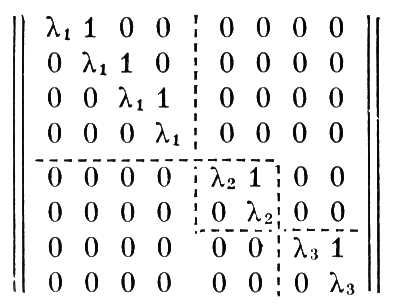
\includegraphics[scale=0.6]{17-1.PNG}
\end{figure}\\

При этом $\lambda_1, ..., \Lambda_n$ - все собственные значения оператора.\\

ДОКАЗАТЕЛЬСТВО ОТДЕЛЬНЫМ ФАЙЛОМ!!!!

\textbf{Собственным подпространством $V^\lambda$} оператора T с собственным значением $\lambda$ называется ядро оператора $(T- \lambda I)$:\\
$V^{\lambda} := Ker(T - \lambda I)$\\
Ненулевые векторы из собственного подпространства называются собственными векторами.\\
\textit{Опр.} \textbf{Корневым подпространством $V^{(\lambda)}$} оператора $T$ с собственным значением $\lambda$ называется ядро оператора $(T- \lambda I)^n$:\\
$V^{(\lambda)}$:=$Ker(T- \lambda I)^n$.\\
\textit{Опр.} \textbf{Минимальный многочлен $m(\lambda)$} оператора T - это ненулевой многочлен минимальной степени, такой что $m_T(T)=0$

\textbf{Линейное рекуррентное соотношение}\\
Линейное рекуррентное уравнение степени k или порядка k - это рекуррентное уравнение в формате: $x_n=A_1x_{n-1}+ A_2x_{n-2}+…+ A_kx_{n-k}$ ($A_n$-константа и $A_k \neq 0$)\\
Предположим, что два упорядоченных линейных рекуррентных соотношения имеют вид:\\
$F_n=AF_{n-1}+BF_{n-2}$, A и B – действительные числа.\\
Характеристическое уравнение для вышеуказанного рекуррентного соотношения: \\
$x^2-Ax-B=0$\\
При поиске корней могут возникать три случая:\\
1.  Если это уравнение преобразуется как $(x - x_1) (x - x_2) = 0$ и оно дает два различных действительных корня $x_1$ и $x_2$, то решение $F_n = ax_1^n + bx_2^n$. (Здесь a и b являются константами)\\
2. Если это уравнение преобразуется как $(x - x_1)^2=0$ и оно дает один действительный корень $x_1$, то решение $F_n = ax_1^n + bnx_1^n$.\\
3. Если уравнение дает два различных комплексных корня, $x_1$ и $x_2$ в полярной форме $x_1 = r \angle \theta$ и $x_2 = r \angle (−\theta )$, то $Fn = r^n (acos (n\theta) + bsin (n\theta))$.\\

Пример. Напишите явную форму $F_n=5F_{n-1}-6F_{n-2}$, где $F_0=1$ и $F_1=4$\\
Решение. Характеристическое уравнение $x^2-5x+6=0$, $x_1=3$ и $x_2=2$. Здесь случай 1. \Rightarrow $F_n=a3^n+b2^n$ \Rightarrow\\
$1=F_0=a3^0+b2^0=a+b$\\
$4=F_1=a3^1+b2^1=3a+2b$\\
Решаем систему, получаем $a=2$ и $b=-1$\\
Ответ: $F_n=2*3^n+(-1)*2^n$


%18 Артем
\item \textbf{Определения: спектр оператора, инвариантные подпространства, прямая сумма подпространств. Пространство с оператором раскладывается в прямую сумму корневых подпространств. Жорданова нормальная форма нильпотентного оператора.}\\
Опр: Набор собственных значений оператора A часто называют его спектром.
Если все собственные значения имеют кратность 1 как корни характеристического
многочлена, то говорят о простом спектре. Таким образом, операторы с простым
спектром диагонализируемы.
Подпространство $W \subset V$ называется инвариантным относительно оператора $A: V \rightarrow V$, если $A(W)\subset W$\\
\\
\\
\textit{Опр.} \textbf{Спектр оператора} $T: spec(T) = \{ \lambda \in {C} | V^{\lambda} \neq {0}\}$ (=множество собственных чисел)\\
${U} \subset {V}$ - \textbf{инвариантное подпространство}, если ${T}(u) \subset U (T|_{U}: {U} \rightarrow {U})$\\
\textbf{Прямая сумма}: ${U},{W} \subset {V}; {V} = {U} \oplus {W} \Leftrightarrow$ каждый $v \in {V}$ единственным образом представим в виде $u+w$, где $u \in {U}, w \in {W}: v=u+w$\\
${V} = {U} \oplus {W} \Leftrightarrow$\\
(1) существует представление $v=u+w$ для всех $v \in {V}$\\
(2) ${U} \cap {W} = {0}$ \\
\textit{\textbf{Теорема.}} ${V} = \oplus {V}^{(\lambda)}$, причем каждое корневое подпространство инвариантно относительно оператора ${T}$\\
Прямая сумма $u,w\subset V$\\
$V=u\oplus{w}$  равносильно каждый $v \in V$ единственным образом представим в ввиде $v= u+w$ где  $u \in U , \  w \in W$ 
$V = U \oplus{W} \Leftrightarrow$ \\
(1) существует представление $v=u+w$ \\
(2) $U \bigcap W = {0}$ \\
$V= R^{2} = {x,y}$\\
$U={y=0}$\\
$W={x=0}$\\
${V}^{(\lambda)} = \oplus {V}^{(\lambda)}_{i}$}
Нильпотентные операторы. Нормальный вид \\
Оператор A называется нильпотентным, если A^k=O для некоторого k. Минимальное число k, для которогоA^k=O, называется степенью нильпотентности оператора A.\\
Рассмотрим оператор A, заданный в базисе $e_1,...,e_n$ (над диагональю стоят единицы, а на остальных местах — нули). Действие этого оператора на базисные векторы описывается схемой $e_n \rightarrow e_{n-1} \rightarrow ... \rightarrow e_1 \rightarrow 0$.Отсюда видно, чтоAn=O, т.е. операторAнильпотентен и имеет степень n.
Пусть $A:V→V$— нильпотентный оператор, причём $dimV=n$. Тогда \\
а) единственным собственным значением оператора A является 0;\\
б)оператор A диагонализируем тогда и только тогда, когда A=O;\\
в)An=O, т.е. степень нильпотентности A не превосходит $n= dimV$
\
\end{enumerate}


\end{document}
